\documentclass[12pt]{article}
\usepackage[utf8]{inputenc}
\usepackage[T1]{fontenc}
\usepackage{mathptmx}
\usepackage[margin=1in]{geometry}
\usepackage{setspace}
\usepackage{amsmath,amssymb}
\usepackage{booktabs}
\usepackage{graphicx}
\usepackage{siunitx}
\usepackage[hidelinks]{hyperref}
\usepackage{xcolor}
\usepackage{microtype}
\usepackage{caption}
\usepackage{pdflscape}
\usepackage[mathlines]{lineno}
\captionsetup{justification=raggedright,singlelinecheck=false}
\graphicspath{{./}}
\newcommand{\CI}[2]{(95\%\ CI #1, #2)}
\newcommand{\tbd}[1]{\textcolor{red}{[#1]}}
% generated by raw_derivation_summary.R; do not edit
\newcommand{\rawMode}{prefix}
\newcommand{\rawNsample}{997}
\newcommand{\rawNcomplete}{1787}
\newcommand{\rawPrefixR}{1000}
\newcommand{\rawPaxpredmSriMean}{58.1}
\newcommand{\rawPaxpredmSriSd}{17.6}
\newcommand{\rawPaxpredmSriMedian}{61.3}
\newcommand{\rawPaxpredmTransDay}{17.8}
\newcommand{\rawPaxpredmSleepMinDay}{471}
\newcommand{\rawPaxpredmMissMask}{0.0}
\newcommand{\rawPaxpredmSriBMean}{58.1}
\newcommand{\rawPaxpredmPctExclB}{0.0}
\newcommand{\rawGgirSibSriMean}{70.2}
\newcommand{\rawGgirSibSriSd}{12.0}
\newcommand{\rawGgirSibSriMedian}{72.2}
\newcommand{\rawGgirSibTransDay}{19.5}
\newcommand{\rawGgirSibSleepMinDay}{336}
\newcommand{\rawGgirSibMissMask}{1.3}
\newcommand{\rawGgirSibSriBMean}{69.3}
\newcommand{\rawGgirSibPctExclB}{0.3}
\newcommand{\rawGgirSibDiffMean}{12.1}
\newcommand{\rawGgirSibDiffLo}{11.3}
\newcommand{\rawGgirSibDiffHi}{12.9}
\newcommand{\rawGgirSibAgreeAll}{87.8}
\newcommand{\rawGgirSibKappaAll}{0.74}
\newcommand{\rawGgirSibKappaAllLo}{0.73}
\newcommand{\rawGgirSibKappaAllHi}{0.74}
\newcommand{\rawGgirSibDmissAll}{1.3}
\newcommand{\rawGgirSibAgreeIsm}{75.4}
\newcommand{\rawGgirSibKappaIsm}{0.48}
\newcommand{\rawGgirSibKappaIsmLo}{0.47}
\newcommand{\rawGgirSibKappaIsmHi}{0.49}
\newcommand{\rawGgirSibDmissIsm}{3.0}
\newcommand{\rawGgirSibAgreeNon}{95.6}
\newcommand{\rawGgirSibKappaNon}{0.41}
\newcommand{\rawGgirSibKappaNonLo}{0.39}
\newcommand{\rawGgirSibKappaNonHi}{0.43}
\newcommand{\rawGgirSibDmissNon}{0.1}
\newcommand{\rawGgirSptSriMean}{75.8}
\newcommand{\rawGgirSptSriSd}{15.1}
\newcommand{\rawGgirSptSriMedian}{79.5}
\newcommand{\rawGgirSptTransDay}{2.0}
\newcommand{\rawGgirSptSleepMinDay}{386}
\newcommand{\rawGgirSptMissMask}{1.3}
\newcommand{\rawGgirSptSriBMean}{75.4}
\newcommand{\rawGgirSptPctExclB}{0.3}
\newcommand{\rawGgirSptDiffMean}{17.7}
\newcommand{\rawGgirSptDiffLo}{16.9}
\newcommand{\rawGgirSptDiffHi}{18.5}
\newcommand{\rawGgirSptAgreeAll}{88.2}
\newcommand{\rawGgirSptKappaAll}{0.75}
\newcommand{\rawGgirSptKappaAllLo}{0.74}
\newcommand{\rawGgirSptKappaAllHi}{0.76}
\newcommand{\rawGgirSptDmissAll}{1.3}
\newcommand{\rawGgirSptAgreeIsm}{78.4}
\newcommand{\rawGgirSptKappaIsm}{0.50}
\newcommand{\rawGgirSptKappaIsmLo}{0.49}
\newcommand{\rawGgirSptKappaIsmHi}{0.52}
\newcommand{\rawGgirSptDmissIsm}{3.0}
\newcommand{\rawGgirSptAgreeNon}{94.5}
\newcommand{\rawGgirSptKappaNon}{0.42}
\newcommand{\rawGgirSptKappaNonLo}{0.40}
\newcommand{\rawGgirSptKappaNonHi}{0.43}
\newcommand{\rawGgirSptDmissNon}{0.1}
\newcommand{\rawSwanSriMean}{68.3}
\newcommand{\rawSwanSriSd}{16.0}
\newcommand{\rawSwanSriMedian}{71.4}
\newcommand{\rawSwanTransDay}{3.0}
\newcommand{\rawSwanSleepMinDay}{365}
\newcommand{\rawSwanMissMask}{0.8}
\newcommand{\rawSwanSriBMean}{67.5}
\newcommand{\rawSwanPctExclB}{0.0}
\newcommand{\rawSwanDiffMean}{10.1}
\newcommand{\rawSwanDiffLo}{9.5}
\newcommand{\rawSwanDiffHi}{10.8}
\newcommand{\rawSwanAgreeAll}{89.4}
\newcommand{\rawSwanKappaAll}{0.77}
\newcommand{\rawSwanKappaAllLo}{0.76}
\newcommand{\rawSwanKappaAllHi}{0.77}
\newcommand{\rawSwanDmissAll}{0.8}
\newcommand{\rawSwanAgreeIsm}{79.9}
\newcommand{\rawSwanKappaIsm}{0.54}
\newcommand{\rawSwanKappaIsmLo}{0.53}
\newcommand{\rawSwanKappaIsmHi}{0.55}
\newcommand{\rawSwanDmissIsm}{1.7}
\newcommand{\rawSwanAgreeNon}{95.4}
\newcommand{\rawSwanKappaNon}{0.45}
\newcommand{\rawSwanKappaNonLo}{0.43}
\newcommand{\rawSwanKappaNonHi}{0.47}
\newcommand{\rawSwanDmissNon}{0.1}
\newcommand{\rawGgirSibBoutSleepMedian}{13.0}
\newcommand{\rawGgirSibBoutSleepPerPerson}{109.9}
\newcommand{\rawGgirSibBoutWakeMedian}{6.0}
\newcommand{\rawGgirSibBoutWakePerPerson}{306.9}
\newcommand{\rawGgirSptBoutSleepMedian}{13.0}
\newcommand{\rawGgirSptBoutSleepPerPerson}{111.6}
\newcommand{\rawGgirSptBoutWakeMedian}{10.0}
\newcommand{\rawGgirSptBoutWakePerPerson}{226.6}
\newcommand{\rawPaxpredmBoutSleepMedian}{12.0}
\newcommand{\rawPaxpredmBoutSleepPerPerson}{148.7}
\newcommand{\rawPaxpredmBoutWakeMedian}{8.0}
\newcommand{\rawPaxpredmBoutWakePerPerson}{224.5}
\newcommand{\rawSwanBoutSleepMedian}{17.0}
\newcommand{\rawSwanBoutSleepPerPerson}{89.3}
\newcommand{\rawSwanBoutWakeMedian}{10.0}
\newcommand{\rawSwanBoutWakePerPerson}{252.0}

% generated by raw_derivation_models.R; do not edit
\newcommand{\rawModelN}{997}
\newcommand{\rawPaxpredmMAEst}{0.920}
\newcommand{\rawPaxpredmMALo}{0.871}
\newcommand{\rawPaxpredmMAHi}{0.968}
\newcommand{\rawPaxpredmMADSri}{42.9}
\newcommand{\rawPaxpredmMAPerTenEst}{-1.9}
\newcommand{\rawPaxpredmMAPerTenLo}{-3.2}
\newcommand{\rawPaxpredmMAPerTenHi}{-0.8}
\newcommand{\rawPaxpredmMBEst}{0.952}
\newcommand{\rawPaxpredmMBLo}{0.907}
\newcommand{\rawPaxpredmMBHi}{0.996}
\newcommand{\rawPaxpredmMBDSri}{42.9}
\newcommand{\rawPaxpredmMBPerTenEst}{-1.1}
\newcommand{\rawPaxpredmMBPerTenLo}{-2.2}
\newcommand{\rawPaxpredmMBPerTenHi}{-0.1}
\newcommand{\rawPaxpredmMCrefEst}{1.014}
\newcommand{\rawPaxpredmMCrefLo}{0.957}
\newcommand{\rawPaxpredmMCrefHi}{1.067}
\newcommand{\rawPaxpredmMCrefDSri}{42.9}
\newcommand{\rawPaxpredmMCrefPerTenEst}{+0.3}
\newcommand{\rawPaxpredmMCrefPerTenLo}{-1.0}
\newcommand{\rawPaxpredmMCrefPerTenHi}{+1.5}
\newcommand{\rawPaxpredmMCotherEst}{0.888}
\newcommand{\rawPaxpredmMCotherLo}{0.819}
\newcommand{\rawPaxpredmMCotherHi}{0.951}
\newcommand{\rawPaxpredmMCotherDSri}{42.9}
\newcommand{\rawPaxpredmMCotherPerTenEst}{-2.7}
\newcommand{\rawPaxpredmMCotherPerTenLo}{-4.6}
\newcommand{\rawPaxpredmMCotherPerTenHi}{-1.2}
\newcommand{\rawGgirSibMAEst}{0.969}
\newcommand{\rawGgirSibMALo}{0.925}
\newcommand{\rawGgirSibMAHi}{1.006}
\newcommand{\rawGgirSibMADSri}{26.5}
\newcommand{\rawGgirSibMAPerTenEst}{-1.2}
\newcommand{\rawGgirSibMAPerTenLo}{-2.9}
\newcommand{\rawGgirSibMAPerTenHi}{+0.2}
\newcommand{\rawGgirSibMBEst}{1.004}
\newcommand{\rawGgirSibMBLo}{0.955}
\newcommand{\rawGgirSibMBHi}{1.041}
\newcommand{\rawGgirSibMBDSri}{26.5}
\newcommand{\rawGgirSibMBPerTenEst}{+0.2}
\newcommand{\rawGgirSibMBPerTenLo}{-1.7}
\newcommand{\rawGgirSibMBPerTenHi}{+1.5}
\newcommand{\rawGgirSibMCrefEst}{1.050}
\newcommand{\rawGgirSibMCrefLo}{0.987}
\newcommand{\rawGgirSibMCrefHi}{1.106}
\newcommand{\rawGgirSibMCrefDSri}{26.5}
\newcommand{\rawGgirSibMCrefPerTenEst}{+1.9}
\newcommand{\rawGgirSibMCrefPerTenLo}{-0.5}
\newcommand{\rawGgirSibMCrefPerTenHi}{+3.9}
\newcommand{\rawGgirSibMCotherEst}{0.967}
\newcommand{\rawGgirSibMCotherLo}{0.904}
\newcommand{\rawGgirSibMCotherHi}{1.016}
\newcommand{\rawGgirSibMCotherDSri}{26.5}
\newcommand{\rawGgirSibMCotherPerTenEst}{-1.3}
\newcommand{\rawGgirSibMCotherPerTenLo}{-3.7}
\newcommand{\rawGgirSibMCotherPerTenHi}{+0.6}
\newcommand{\rawGgirSptMAEst}{0.964}
\newcommand{\rawGgirSptMALo}{0.926}
\newcommand{\rawGgirSptMAHi}{1.006}
\newcommand{\rawGgirSptMADSri}{33.6}
\newcommand{\rawGgirSptMAPerTenEst}{-1.1}
\newcommand{\rawGgirSptMAPerTenLo}{-2.3}
\newcommand{\rawGgirSptMAPerTenHi}{+0.2}
\newcommand{\rawGgirSptMBEst}{0.999}
\newcommand{\rawGgirSptMBLo}{0.952}
\newcommand{\rawGgirSptMBHi}{1.037}
\newcommand{\rawGgirSptMBDSri}{33.6}
\newcommand{\rawGgirSptMBPerTenEst}{0.0}
\newcommand{\rawGgirSptMBPerTenLo}{-1.4}
\newcommand{\rawGgirSptMBPerTenHi}{+1.1}
\newcommand{\rawGgirSptMCrefEst}{1.028}
\newcommand{\rawGgirSptMCrefLo}{0.966}
\newcommand{\rawGgirSptMCrefHi}{1.083}
\newcommand{\rawGgirSptMCrefDSri}{33.6}
\newcommand{\rawGgirSptMCrefPerTenEst}{+0.8}
\newcommand{\rawGgirSptMCrefPerTenLo}{-1.0}
\newcommand{\rawGgirSptMCrefPerTenHi}{+2.4}
\newcommand{\rawGgirSptMCotherEst}{0.973}
\newcommand{\rawGgirSptMCotherLo}{0.917}
\newcommand{\rawGgirSptMCotherHi}{1.021}
\newcommand{\rawGgirSptMCotherDSri}{33.6}
\newcommand{\rawGgirSptMCotherPerTenEst}{-0.8}
\newcommand{\rawGgirSptMCotherPerTenLo}{-2.5}
\newcommand{\rawGgirSptMCotherPerTenHi}{+0.6}
\newcommand{\rawSwanMAEst}{0.957}
\newcommand{\rawSwanMALo}{0.913}
\newcommand{\rawSwanMAHi}{0.994}
\newcommand{\rawSwanMADSri}{37.9}
\newcommand{\rawSwanMAPerTenEst}{-1.2}
\newcommand{\rawSwanMAPerTenLo}{-2.4}
\newcommand{\rawSwanMAPerTenHi}{-0.2}
\newcommand{\rawSwanMBEst}{0.993}
\newcommand{\rawSwanMBLo}{0.951}
\newcommand{\rawSwanMBHi}{1.025}
\newcommand{\rawSwanMBDSri}{37.9}
\newcommand{\rawSwanMBPerTenEst}{-0.2}
\newcommand{\rawSwanMBPerTenLo}{-1.3}
\newcommand{\rawSwanMBPerTenHi}{+0.7}
\newcommand{\rawSwanMCrefEst}{1.028}
\newcommand{\rawSwanMCrefLo}{0.967}
\newcommand{\rawSwanMCrefHi}{1.070}
\newcommand{\rawSwanMCrefDSri}{37.9}
\newcommand{\rawSwanMCrefPerTenEst}{+0.7}
\newcommand{\rawSwanMCrefPerTenLo}{-0.9}
\newcommand{\rawSwanMCrefPerTenHi}{+1.8}
\newcommand{\rawSwanMCotherEst}{0.956}
\newcommand{\rawSwanMCotherLo}{0.900}
\newcommand{\rawSwanMCotherHi}{1.012}
\newcommand{\rawSwanMCotherDSri}{37.9}
\newcommand{\rawSwanMCotherPerTenEst}{-1.2}
\newcommand{\rawSwanMCotherPerTenLo}{-2.7}
\newcommand{\rawSwanMCotherPerTenHi}{+0.3}
\newcommand{\rawGgirSibMARatioEst}{1.053}
\newcommand{\rawGgirSibMARatioLo}{1.020}
\newcommand{\rawGgirSibMARatioHi}{1.083}
\newcommand{\rawGgirSibMBRatioEst}{1.055}
\newcommand{\rawGgirSibMBRatioLo}{1.014}
\newcommand{\rawGgirSibMBRatioHi}{1.096}
\newcommand{\rawGgirSibMCrefRatioEst}{1.036}
\newcommand{\rawGgirSibMCrefRatioLo}{0.989}
\newcommand{\rawGgirSibMCrefRatioHi}{1.075}
\newcommand{\rawGgirSibMCotherRatioEst}{1.089}
\newcommand{\rawGgirSibMCotherRatioLo}{1.038}
\newcommand{\rawGgirSibMCotherRatioHi}{1.144}
\newcommand{\rawGgirSptMARatioEst}{1.048}
\newcommand{\rawGgirSptMARatioLo}{1.015}
\newcommand{\rawGgirSptMARatioHi}{1.076}
\newcommand{\rawGgirSptMBRatioEst}{1.049}
\newcommand{\rawGgirSptMBRatioLo}{1.012}
\newcommand{\rawGgirSptMBRatioHi}{1.084}
\newcommand{\rawGgirSptMCrefRatioEst}{1.014}
\newcommand{\rawGgirSptMCrefRatioLo}{0.971}
\newcommand{\rawGgirSptMCrefRatioHi}{1.055}
\newcommand{\rawGgirSptMCotherRatioEst}{1.096}
\newcommand{\rawGgirSptMCotherRatioLo}{1.051}
\newcommand{\rawGgirSptMCotherRatioHi}{1.150}
\newcommand{\rawSwanMARatioEst}{1.040}
\newcommand{\rawSwanMARatioLo}{1.009}
\newcommand{\rawSwanMARatioHi}{1.068}
\newcommand{\rawSwanMBRatioEst}{1.043}
\newcommand{\rawSwanMBRatioLo}{1.010}
\newcommand{\rawSwanMBRatioHi}{1.077}
\newcommand{\rawSwanMCrefRatioEst}{1.014}
\newcommand{\rawSwanMCrefRatioLo}{0.979}
\newcommand{\rawSwanMCrefRatioHi}{1.048}
\newcommand{\rawSwanMCotherRatioEst}{1.078}
\newcommand{\rawSwanMCotherRatioLo}{1.023}
\newcommand{\rawSwanMCotherRatioHi}{1.138}

% generated by raw_derivation_models.R; do not edit
\newcommand{\rawModelNB}{994}
\newcommand{\rawPaxpredmMABEst}{0.920}
\newcommand{\rawPaxpredmMABLo}{0.882}
\newcommand{\rawPaxpredmMABHi}{0.965}
\newcommand{\rawPaxpredmMABDSri}{43.0}
\newcommand{\rawPaxpredmMABPerTenEst}{-1.9}
\newcommand{\rawPaxpredmMABPerTenLo}{-2.9}
\newcommand{\rawPaxpredmMABPerTenHi}{-0.8}
\newcommand{\rawPaxpredmMBBEst}{0.953}
\newcommand{\rawPaxpredmMBBLo}{0.909}
\newcommand{\rawPaxpredmMBBHi}{0.998}
\newcommand{\rawPaxpredmMBBDSri}{43.0}
\newcommand{\rawPaxpredmMBBPerTenEst}{-1.1}
\newcommand{\rawPaxpredmMBBPerTenLo}{-2.2}
\newcommand{\rawPaxpredmMBBPerTenHi}{-0.0}
\newcommand{\rawPaxpredmMCrefBEst}{1.017}
\newcommand{\rawPaxpredmMCrefBLo}{0.959}
\newcommand{\rawPaxpredmMCrefBHi}{1.071}
\newcommand{\rawPaxpredmMCrefBDSri}{43.0}
\newcommand{\rawPaxpredmMCrefBPerTenEst}{+0.4}
\newcommand{\rawPaxpredmMCrefBPerTenLo}{-1.0}
\newcommand{\rawPaxpredmMCrefBPerTenHi}{+1.6}
\newcommand{\rawPaxpredmMCotherBEst}{0.887}
\newcommand{\rawPaxpredmMCotherBLo}{0.821}
\newcommand{\rawPaxpredmMCotherBHi}{0.936}
\newcommand{\rawPaxpredmMCotherBDSri}{43.0}
\newcommand{\rawPaxpredmMCotherBPerTenEst}{-2.7}
\newcommand{\rawPaxpredmMCotherBPerTenLo}{-4.5}
\newcommand{\rawPaxpredmMCotherBPerTenHi}{-1.5}
\newcommand{\rawGgirSibMABEst}{0.974}
\newcommand{\rawGgirSibMABLo}{0.936}
\newcommand{\rawGgirSibMABHi}{1.013}
\newcommand{\rawGgirSibMABDSri}{25.8}
\newcommand{\rawGgirSibMABPerTenEst}{-1.0}
\newcommand{\rawGgirSibMABPerTenLo}{-2.5}
\newcommand{\rawGgirSibMABPerTenHi}{+0.5}
\newcommand{\rawGgirSibMBBEst}{1.009}
\newcommand{\rawGgirSibMBBLo}{0.969}
\newcommand{\rawGgirSibMBBHi}{1.045}
\newcommand{\rawGgirSibMBBDSri}{25.8}
\newcommand{\rawGgirSibMBBPerTenEst}{+0.3}
\newcommand{\rawGgirSibMBBPerTenLo}{-1.2}
\newcommand{\rawGgirSibMBBPerTenHi}{+1.7}
\newcommand{\rawGgirSibMCrefBEst}{1.053}
\newcommand{\rawGgirSibMCrefBLo}{0.994}
\newcommand{\rawGgirSibMCrefBHi}{1.105}
\newcommand{\rawGgirSibMCrefBDSri}{25.8}
\newcommand{\rawGgirSibMCrefBPerTenEst}{+2.0}
\newcommand{\rawGgirSibMCrefBPerTenLo}{-0.2}
\newcommand{\rawGgirSibMCrefBPerTenHi}{+4.0}
\newcommand{\rawGgirSibMCotherBEst}{0.975}
\newcommand{\rawGgirSibMCotherBLo}{0.924}
\newcommand{\rawGgirSibMCotherBHi}{1.033}
\newcommand{\rawGgirSibMCotherBDSri}{25.8}
\newcommand{\rawGgirSibMCotherBPerTenEst}{-1.0}
\newcommand{\rawGgirSibMCotherBPerTenLo}{-3.0}
\newcommand{\rawGgirSibMCotherBPerTenHi}{+1.3}
\newcommand{\rawGgirSptMABEst}{0.965}
\newcommand{\rawGgirSptMABLo}{0.927}
\newcommand{\rawGgirSptMABHi}{1.001}
\newcommand{\rawGgirSptMABDSri}{33.8}
\newcommand{\rawGgirSptMABPerTenEst}{-1.0}
\newcommand{\rawGgirSptMABPerTenLo}{-2.2}
\newcommand{\rawGgirSptMABPerTenHi}{+0.0}
\newcommand{\rawGgirSptMBBEst}{1.001}
\newcommand{\rawGgirSptMBBLo}{0.960}
\newcommand{\rawGgirSptMBBHi}{1.036}
\newcommand{\rawGgirSptMBBDSri}{33.8}
\newcommand{\rawGgirSptMBBPerTenEst}{+0.0}
\newcommand{\rawGgirSptMBBPerTenLo}{-1.2}
\newcommand{\rawGgirSptMBBPerTenHi}{+1.0}
\newcommand{\rawGgirSptMCrefBEst}{1.028}
\newcommand{\rawGgirSptMCrefBLo}{0.968}
\newcommand{\rawGgirSptMCrefBHi}{1.082}
\newcommand{\rawGgirSptMCrefBDSri}{33.8}
\newcommand{\rawGgirSptMCrefBPerTenEst}{+0.8}
\newcommand{\rawGgirSptMCrefBPerTenLo}{-1.0}
\newcommand{\rawGgirSptMCrefBPerTenHi}{+2.4}
\newcommand{\rawGgirSptMCotherBEst}{0.976}
\newcommand{\rawGgirSptMCotherBLo}{0.925}
\newcommand{\rawGgirSptMCotherBHi}{1.023}
\newcommand{\rawGgirSptMCotherBDSri}{33.8}
\newcommand{\rawGgirSptMCotherBPerTenEst}{-0.7}
\newcommand{\rawGgirSptMCotherBPerTenLo}{-2.3}
\newcommand{\rawGgirSptMCotherBPerTenHi}{+0.7}
\newcommand{\rawSwanMABEst}{0.961}
\newcommand{\rawSwanMABLo}{0.924}
\newcommand{\rawSwanMABHi}{0.997}
\newcommand{\rawSwanMABDSri}{38.5}
\newcommand{\rawSwanMABPerTenEst}{-1.0}
\newcommand{\rawSwanMABPerTenLo}{-2.0}
\newcommand{\rawSwanMABPerTenHi}{-0.1}
\newcommand{\rawSwanMBBEst}{0.997}
\newcommand{\rawSwanMBBLo}{0.962}
\newcommand{\rawSwanMBBHi}{1.032}
\newcommand{\rawSwanMBBDSri}{38.5}
\newcommand{\rawSwanMBBPerTenEst}{-0.1}
\newcommand{\rawSwanMBBPerTenLo}{-1.0}
\newcommand{\rawSwanMBBPerTenHi}{+0.8}
\newcommand{\rawSwanMCrefBEst}{1.033}
\newcommand{\rawSwanMCrefBLo}{0.979}
\newcommand{\rawSwanMCrefBHi}{1.079}
\newcommand{\rawSwanMCrefBDSri}{38.5}
\newcommand{\rawSwanMCrefBPerTenEst}{+0.8}
\newcommand{\rawSwanMCrefBPerTenLo}{-0.6}
\newcommand{\rawSwanMCrefBPerTenHi}{+2.0}
\newcommand{\rawSwanMCotherBEst}{0.962}
\newcommand{\rawSwanMCotherBLo}{0.906}
\newcommand{\rawSwanMCotherBHi}{1.020}
\newcommand{\rawSwanMCotherBDSri}{38.5}
\newcommand{\rawSwanMCotherBPerTenEst}{-1.0}
\newcommand{\rawSwanMCotherBPerTenLo}{-2.5}
\newcommand{\rawSwanMCotherBPerTenHi}{+0.5}
\newcommand{\rawGgirSibMARatioBEst}{1.059}
\newcommand{\rawGgirSibMARatioBLo}{1.030}
\newcommand{\rawGgirSibMARatioBHi}{1.091}
\newcommand{\rawGgirSibMBRatioBEst}{1.058}
\newcommand{\rawGgirSibMBRatioBLo}{1.023}
\newcommand{\rawGgirSibMBRatioBHi}{1.102}
\newcommand{\rawGgirSibMCrefRatioBEst}{1.035}
\newcommand{\rawGgirSibMCrefRatioBLo}{0.995}
\newcommand{\rawGgirSibMCrefRatioBHi}{1.075}
\newcommand{\rawGgirSibMCotherRatioBEst}{1.099}
\newcommand{\rawGgirSibMCotherRatioBLo}{1.055}
\newcommand{\rawGgirSibMCotherRatioBHi}{1.167}
\newcommand{\rawGgirSptMARatioBEst}{1.049}
\newcommand{\rawGgirSptMARatioBLo}{1.020}
\newcommand{\rawGgirSptMARatioBHi}{1.076}
\newcommand{\rawGgirSptMBRatioBEst}{1.049}
\newcommand{\rawGgirSptMBRatioBLo}{1.016}
\newcommand{\rawGgirSptMBRatioBHi}{1.089}
\newcommand{\rawGgirSptMCrefRatioBEst}{1.011}
\newcommand{\rawGgirSptMCrefRatioBLo}{0.971}
\newcommand{\rawGgirSptMCrefRatioBHi}{1.044}
\newcommand{\rawGgirSptMCotherRatioBEst}{1.100}
\newcommand{\rawGgirSptMCotherRatioBLo}{1.047}
\newcommand{\rawGgirSptMCotherRatioBHi}{1.155}
\newcommand{\rawSwanMARatioBEst}{1.045}
\newcommand{\rawSwanMARatioBLo}{1.017}
\newcommand{\rawSwanMARatioBHi}{1.072}
\newcommand{\rawSwanMBRatioBEst}{1.046}
\newcommand{\rawSwanMBRatioBLo}{1.015}
\newcommand{\rawSwanMBRatioBHi}{1.085}
\newcommand{\rawSwanMCrefRatioBEst}{1.016}
\newcommand{\rawSwanMCrefRatioBLo}{0.983}
\newcommand{\rawSwanMCrefRatioBHi}{1.049}
\newcommand{\rawSwanMCotherRatioBEst}{1.084}
\newcommand{\rawSwanMCotherRatioBLo}{1.028}
\newcommand{\rawSwanMCotherRatioBHi}{1.152}

% generated by compute_timing_summary.py; do not edit
\newcommand{\rawComputeN}{997}
\newcommand{\rawComputeDays}{3.2}
\newcommand{\rawComputeHours}{384}
\newcommand{\rawComputeMedianMin}{22}
\newcommand{\rawComputeStart}{15 October 2026}
\newcommand{\rawComputeEnd}{18 October 2026}
\newcommand{\rawComputeMacN}{625}
\newcommand{\rawComputeMacHours}{213}
\newcommand{\rawComputeMacMedianMin}{20}
\newcommand{\rawComputeAwsN}{249}
\newcommand{\rawComputeAwsHours}{119}
\newcommand{\rawComputeAwsMedianMin}{29}
\newcommand{\rawComputeMOneN}{27}
\newcommand{\rawComputeMOneHours}{11}
\newcommand{\rawComputeMOneMedianMin}{25}
\newcommand{\rawComputeHetznerN}{70}
\newcommand{\rawComputeHetznerHours}{29}
\newcommand{\rawComputeHetznerMedianMin}{25}
\newcommand{\rawComputeVultrN}{26}
\newcommand{\rawComputeVultrHours}{12}
\newcommand{\rawComputeVultrMedianMin}{28}

% generated by make_extra_numbers.R; numbers of the derivation sample
\newcommand{\rawNexcl}{3}
\newcommand{\rawExclSeqn}{83452, 69334, 64226}
\newcommand{\rawNexclAll}{7}
\newcommand{\rawSeed}{20261016}

% generated by m4_tables.R; do not edit
\newcommand{\mfourMaxDiffGgir}{0.013}
\newcommand{\mfourMaxDiffSleepregFive}{0.064}
\newcommand{\mfourMaxDiffSleepregThree}{0.026}
\newcommand{\mfourWomenBelowMen}{36 of 36}
\newcommand{\mfourShiftLo}{-0.020}
\newcommand{\mfourShiftHi}{+0.030}
\newcommand{\mfourNhwWomenPubEst}{0.906}
\newcommand{\mfourNhwWomenPubLo}{0.877}
\newcommand{\mfourNhwWomenPubHi}{0.935}
\newcommand{\mfourNhwWomenRelEst}{0.912}
\newcommand{\mfourNhwWomenRelLo}{0.887}
\newcommand{\mfourNhwWomenRelHi}{0.945}
\newcommand{\mfourNhwWomenSptEst}{0.934}
\newcommand{\mfourNhwWomenSptLo}{0.906}
\newcommand{\mfourNhwWomenSptHi}{0.963}
\newcommand{\mfourNhwMenPubEst}{0.968}
\newcommand{\mfourNhwMenPubLo}{0.942}
\newcommand{\mfourNhwMenPubHi}{0.993}
\newcommand{\mfourNhwMenRelEst}{0.975}
\newcommand{\mfourNhwMenRelLo}{0.945}
\newcommand{\mfourNhwMenRelHi}{1.001}
\newcommand{\mfourNhwMenSptEst}{0.983}
\newcommand{\mfourNhwMenSptLo}{0.957}
\newcommand{\mfourNhwMenSptHi}{1.006}
\newcommand{\mfourNhbMenRelEst}{1.035}
\newcommand{\mfourNhbMenRelLo}{0.998}
\newcommand{\mfourNhbMenRelHi}{1.073}
\newcommand{\mfourNhbMenSptEst}{1.047}
\newcommand{\mfourNhbMenSptLo}{1.016}
\newcommand{\mfourNhbMenSptHi}{1.087}
\newcommand{\mfourMexMenRelEst}{1.034}
\newcommand{\mfourMexMenRelLo}{0.994}
\newcommand{\mfourMexMenRelHi}{1.080}
\newcommand{\mfourMexMenSptEst}{1.042}
\newcommand{\mfourMexMenSptLo}{1.010}
\newcommand{\mfourMexMenSptHi}{1.087}
\newcommand{\mfourOthWomenPubEst}{0.868}
\newcommand{\mfourOthWomenPubLo}{0.791}
\newcommand{\mfourOthWomenPubHi}{0.964}
\newcommand{\mfourOthWomenRelEst}{0.887}
\newcommand{\mfourOthWomenRelLo}{0.797}
\newcommand{\mfourOthWomenRelHi}{0.988}
\newcommand{\mfourOthWomenSptEst}{0.882}
\newcommand{\mfourOthWomenSptLo}{0.785}
\newcommand{\mfourOthWomenSptHi}{1.000}
\newcommand{\mfourOthHispMenRelEst}{1.003}
\newcommand{\mfourOthHispMenRelLo}{0.959}
\newcommand{\mfourOthHispMenRelHi}{1.056}
\newcommand{\mfourOthWomenN}{111}
\newcommand{\mfourPubMaxDiffOrig}{0.014}
\newcommand{\mfourRawNmin}{11}
\newcommand{\mfourRawNmax}{226}
\newcommand{\mfourRawWidthMin}{0.13}
\newcommand{\mfourRawWidthMax}{0.88}
\newcommand{\mfourRawWomenBelowMenPaxpredm}{6 of 6}
\newcommand{\mfourRawWomenBelowMenSwan}{6 of 6}
\newcommand{\mfourRawWomenBelowMenSib}{6 of 6}
\newcommand{\mfourRawWomenBelowMenSpt}{6 of 6}
\newcommand{\simTwoTruth}{0.955}
\newcommand{\simTwoNsim}{20}
\newcommand{\simTwoMfMin}{0.936}
\newcommand{\simTwoMfMax}{0.964}
\newcommand{\simTwoCoverNinetyFive}{18}
\newcommand{\simTwoCoverNinetyNine}{20}
\newcommand{\simTwoWidthNinetyFive}{0.036}
\newcommand{\simTwoWidthNinetyNine}{0.046}
\newcommand{\simTwoLoMin}{0.915}
\newcommand{\simTwoHiMax}{0.981}
\newcommand{\simTwoAboveOne}{0}
\newcommand{\simThreeWTruth}{0.922}
\newcommand{\simThreeWNsim}{20}
\newcommand{\simThreeWMfMin}{0.894}
\newcommand{\simThreeWMfMax}{0.942}
\newcommand{\simThreeWCoverNinetyFive}{18}
\newcommand{\simThreeWCoverNinetyNine}{19}
\newcommand{\simThreeWWidthNinetyFive}{0.045}
\newcommand{\simThreeWWidthNinetyNine}{0.056}
\newcommand{\simThreeWLoMin}{0.873}
\newcommand{\simThreeWHiMax}{0.964}
\newcommand{\simThreeWAboveOne}{0}

% generated by raw_models_smoothed.R; do not edit
\newcommand{\rawMajMAEst}{0.938}
\newcommand{\rawMajMALo}{0.895}
\newcommand{\rawMajMAHi}{0.985}
\newcommand{\rawMajMADSri}{44.4}
\newcommand{\rawMajMARatioEst}{1.020}
\newcommand{\rawMajMARatioLo}{1.010}
\newcommand{\rawMajMARatioHi}{1.032}
\newcommand{\rawMajMBEst}{0.970}
\newcommand{\rawMajMBLo}{0.925}
\newcommand{\rawMajMBHi}{1.010}
\newcommand{\rawMajMBDSri}{44.4}
\newcommand{\rawMajMBRatioEst}{1.019}
\newcommand{\rawMajMBRatioLo}{1.007}
\newcommand{\rawMajMBRatioHi}{1.030}
\newcommand{\rawMajMCrefEst}{1.026}
\newcommand{\rawMajMCrefLo}{0.968}
\newcommand{\rawMajMCrefHi}{1.073}
\newcommand{\rawMajMCrefDSri}{44.4}
\newcommand{\rawMajMCrefRatioEst}{1.012}
\newcommand{\rawMajMCrefRatioLo}{1.000}
\newcommand{\rawMajMCrefRatioHi}{1.028}
\newcommand{\rawMajMCotherEst}{0.909}
\newcommand{\rawMajMCotherLo}{0.842}
\newcommand{\rawMajMCotherHi}{0.973}
\newcommand{\rawMajMCotherDSri}{44.4}
\newcommand{\rawMajMCotherRatioEst}{1.024}
\newcommand{\rawMajMCotherRatioLo}{1.005}
\newcommand{\rawMajMCotherRatioHi}{1.041}
\newcommand{\rawGgirsmMAEst}{0.935}
\newcommand{\rawGgirsmMALo}{0.889}
\newcommand{\rawGgirsmMAHi}{0.983}
\newcommand{\rawGgirsmMADSri}{37.4}
\newcommand{\rawGgirsmMARatioEst}{1.016}
\newcommand{\rawGgirsmMARatioLo}{0.997}
\newcommand{\rawGgirsmMARatioHi}{1.036}
\newcommand{\rawGgirsmMBEst}{0.969}
\newcommand{\rawGgirsmMBLo}{0.927}
\newcommand{\rawGgirsmMBHi}{1.015}
\newcommand{\rawGgirsmMBDSri}{37.4}
\newcommand{\rawGgirsmMBRatioEst}{1.018}
\newcommand{\rawGgirsmMBRatioLo}{0.997}
\newcommand{\rawGgirsmMBRatioHi}{1.045}
\newcommand{\rawGgirsmMCrefEst}{1.020}
\newcommand{\rawGgirsmMCrefLo}{0.966}
\newcommand{\rawGgirsmMCrefHi}{1.067}
\newcommand{\rawGgirsmMCrefDSri}{37.4}
\newcommand{\rawGgirsmMCrefRatioEst}{1.006}
\newcommand{\rawGgirsmMCrefRatioLo}{0.982}
\newcommand{\rawGgirsmMCrefRatioHi}{1.036}
\newcommand{\rawGgirsmMCotherEst}{0.918}
\newcommand{\rawGgirsmMCotherLo}{0.850}
\newcommand{\rawGgirsmMCotherHi}{0.989}
\newcommand{\rawGgirsmMCotherDSri}{37.4}
\newcommand{\rawGgirsmMCotherRatioEst}{1.034}
\newcommand{\rawGgirsmMCotherRatioLo}{1.001}
\newcommand{\rawGgirsmMCotherRatioHi}{1.068}
\newcommand{\rawBridgeMAEst}{0.938}
\newcommand{\rawBridgeMALo}{0.894}
\newcommand{\rawBridgeMAHi}{0.981}
\newcommand{\rawBridgeMADSri}{45.9}
\newcommand{\rawBridgeMARatioEst}{1.020}
\newcommand{\rawBridgeMARatioLo}{1.010}
\newcommand{\rawBridgeMARatioHi}{1.029}
\newcommand{\rawBridgeMBEst}{0.970}
\newcommand{\rawBridgeMBLo}{0.926}
\newcommand{\rawBridgeMBHi}{1.013}
\newcommand{\rawBridgeMBDSri}{45.9}
\newcommand{\rawBridgeMBRatioEst}{1.019}
\newcommand{\rawBridgeMBRatioLo}{1.007}
\newcommand{\rawBridgeMBRatioHi}{1.030}
\newcommand{\rawBridgeMCrefEst}{1.027}
\newcommand{\rawBridgeMCrefLo}{0.966}
\newcommand{\rawBridgeMCrefHi}{1.080}
\newcommand{\rawBridgeMCrefDSri}{45.9}
\newcommand{\rawBridgeMCrefRatioEst}{1.014}
\newcommand{\rawBridgeMCrefRatioLo}{1.002}
\newcommand{\rawBridgeMCrefRatioHi}{1.027}
\newcommand{\rawBridgeMCotherEst}{0.910}
\newcommand{\rawBridgeMCotherLo}{0.844}
\newcommand{\rawBridgeMCotherHi}{0.969}
\newcommand{\rawBridgeMCotherDSri}{45.9}
\newcommand{\rawBridgeMCotherRatioEst}{1.025}
\newcommand{\rawBridgeMCotherRatioLo}{1.008}
\newcommand{\rawBridgeMCotherRatioHi}{1.041}
\newcommand{\rawSptMAEst}{0.952}
\newcommand{\rawSptMALo}{0.906}
\newcommand{\rawSptMAHi}{0.996}
\newcommand{\rawSptMADSri}{39.1}
\newcommand{\rawSptMARatioEst}{1.035}
\newcommand{\rawSptMARatioLo}{1.003}
\newcommand{\rawSptMARatioHi}{1.067}
\newcommand{\rawSptMBEst}{0.979}
\newcommand{\rawSptMBLo}{0.936}
\newcommand{\rawSptMBHi}{1.023}
\newcommand{\rawSptMBDSri}{39.1}
\newcommand{\rawSptMBRatioEst}{1.028}
\newcommand{\rawSptMBRatioLo}{0.996}
\newcommand{\rawSptMBRatioHi}{1.068}
\newcommand{\rawSptMCrefEst}{1.012}
\newcommand{\rawSptMCrefLo}{0.947}
\newcommand{\rawSptMCrefHi}{1.068}
\newcommand{\rawSptMCrefDSri}{39.1}
\newcommand{\rawSptMCrefRatioEst}{0.998}
\newcommand{\rawSptMCrefRatioLo}{0.965}
\newcommand{\rawSptMCrefRatioHi}{1.040}
\newcommand{\rawSptMCotherEst}{0.945}
\newcommand{\rawSptMCotherLo}{0.885}
\newcommand{\rawSptMCotherHi}{1.005}
\newcommand{\rawSptMCotherDSri}{39.1}
\newcommand{\rawSptMCotherRatioEst}{1.065}
\newcommand{\rawSptMCotherRatioLo}{1.018}
\newcommand{\rawSptMCotherRatioHi}{1.123}
\newcommand{\rawSmoothedMBMin}{0.969}
\newcommand{\rawSmoothedMBMax}{0.979}


\title{\bfseries Does the choice of Sleep Regularity Index calculator or
sleep/wake input change the conclusions? A re-analysis of the NHANES
2011--2014 sleep regularity--obesity association}
\author{J\"urgen Degenfellner\\[6pt]
\normalsize Institute of Physiotherapy, ZHAW School of Health Sciences,
Winterthur, Switzerland\\
\normalsize Correspondence: degn@zhaw.ch\\
\normalsize ORCID: 0000-0001-6886-4583}
\date{}

\doublespacing
\begin{document}
\linenumbers

\maketitle
\thispagestyle{empty}
\clearpage

\section*{Abstract}

\textbf{Background.} Open-source packages for the Sleep Regularity Index
(SRI) can score the same recording differently. An earlier study
reported an inverse cross-sectional association between the SRI and body mass index (BMI) in
NHANES 2011--2014 from the released sleep/wake classification. The same
data were re-analysed to examine whether that association depends on the
calculator, the structure of the released classification or the derivation
from the raw signal.

\noindent\textbf{Methods.} The released classification of the published sample
($n=7085$) was rebuilt, four smoothed versions were derived,
and the Phillips formula, \texttt{GGIR} and \texttt{sleepreg} were applied to
each. The survey-weighted $\log$-BMI models were refitted and the calculators
tested on synthetic recordings.
For a random sample of \rawPrefixR{} participants the series was derived anew
from the 80\,Hz raw signal with \texttt{GGIR} and with the public SWaN code.

\noindent\textbf{Results.} The rebuilt series correlated $0.96$ with the
published SRI values. The released classification changed
between sleep and wake a median of 16 times per day. Smoothing raised the median SRI from 61 to 68--76. On the same input the calculators agreed to 0.1 points on average. As a percentage difference in BMI between the top and bottom SRI quintile, the fully adjusted multiplication factor was $-4.5\%$ for the released series and $-2.8\%$ to $-3.7\%$ after smoothing. SWaN rerun on the raw signal of the random sample changed state \rawSwanTransDay{} times per day (mean) against \rawPaxpredmTransDay{} for the release. The three series derived anew with \texttt{GGIR} and SWaN scored \rawSwanDiffMean{} to \rawGgirSptDiffMean{} points higher than the release. In this sample the same percentage difference moved from $-4.8\%$ for the released classification to between $-0.7\%$ and $+0.4\%$ for the derived series. In a
synthetic recording with an SRI of $68.75$, deleting one day instead of
marking it as missing made \texttt{sleepreg} return $35.18$ without warning. Its default minimum of five valid days left 48\% of participants without a
value.

\noindent\textbf{Conclusions.} The SRI level depended on the input and only
marginally on the calculator. The released classification is
more fragmented than a new classification of the same signal with the same algorithm's public code. The inverse association with BMI weakened with every smoothed and newly derived input. Reports should describe the
derivation and smoothing of the series, the treatment of gaps, the minimum-day rule and the remaining sample. The code should be archived.

\vspace{0.6em}
\noindent\textbf{Keywords:} sleep regularity index; NHANES; accelerometry; wearable monitors; \texttt{GGIR};
\texttt{sleepreg}; measurement error; reproducibility; missing data

\clearpage

\section{Background}

The Sleep Regularity Index [1] (SRI) measures the
day-to-day similarity of a person's sleep/wake pattern. For every pair of
epochs exactly 24\,h apart it records whether the state is the same. The index is $-100$ plus $200$ times the proportion of agreeing pairs. Identical
days score $100$ and a random pattern approximately $0$ [2].

Czeisler et al. [20] compared the two most widely used open-source
calculators, \texttt{sleepreg} [3] and \texttt{GGIR}
[4, 5], in 73{,}794 adults of the UK
Biobank. The packages gave markedly different scores and, through the calculator
alone, different prospective associations with mortality, type~2 diabetes and atrial fibrillation. The authors proposed the Reporting Items for Regularity
Indices (RIRI).

An earlier study [6] reported an inverse
cross-sectional association between the SRI and body mass index (BMI) in the National Health and Nutrition Examination Survey (NHANES) 2011--2014 ($n=7085$), more clearly in women. It computed the SRI with its own
implementation of the Phillips formula from the minute-level sleep/wake
classification that NHANES distributes with its accelerometer data (the
variable \texttt{PAXPREDM}). Its results therefore rest on one calculator and one input.

Reported SRI values for the same NHANES accelerometry include a median of $78.1$ [7], a mean of $63.0$ [8] and the median of $63.9$ (unweighted $61.5$) of the earlier study. Cohorts whose epoch series come from a
sleep-period detection step report medians of $81$ [3] and
$74.7$ [9], whereas the NHANES classification is
released minute by minute without such a step [10]. An SRI pipeline has two steps that
can move the score, the derivation of the epoch-level series from the raw
signal and the computation of the index from that series. Czeisler et al. [20] held the first step fixed. A released classification allows the
complementary design, in which the same series is smoothed in defined ways and
every version is passed to every calculator. NHANES has also
released the raw 80\,Hz signal [11],
so that the first step can be repeated, with the sleep detection of
\texttt{GGIR} [5, 12] and with the public code of SWaN (sleep-wear, wake-wear and nonwear classifier), the algorithm that its developers report to have generated the released
classification [10].

The re-analysis therefore asked whether the published values can be rebuilt from the public files, whether the structure of the released classification
sets the level of the SRI, whether the calculators differ once they receive
the same series, whether the published SRI--BMI association keeps its
direction and size under smoothed and under newly derived series, and how a
recording gap passed to a package changes its result.

\section{Methods}

\subsection{Rebuilding the sleep/wake series}
\label{sec:rebuild}
The minute-level sleep/wake series of the earlier study was rebuilt from the
NHANES 2011--2014 minute files. \texttt{PAXPREDM} was recoded to sleep, wake or missing (non-wear and unknown). The published inclusion filters were then applied: full-minute observations, no quality flags, at least 3 days with less
than 120\,min of non-wear, days of exactly 1440 minutes, at least 3
consecutive days including a weekend day, and less than 30\% missing minutes
per participant. The series of each participant was then laid out as one
continuous timeline with one value per minute from monitor placement to the
end of the last retained day, every day starting at 00:00. Minutes and days
that the filters had removed stayed in this timeline as missing values and
were not deleted. Neither package checks whether successive days of a series are consecutive in time. When a day is deleted, \texttt{GGIR} pairs the date before the gap with the next date present, \texttt{sleepreg} carries the last state over the gap, and neither gives a warning (Section~\ref{sec:gapresults}). A day marked as missing is left out of the comparison. The Phillips formula on this shared timeline of the 7085 participants (it returns
a value for 7076 of them) was the same-input baseline. Its relation to the published values is described in Supplementary Section~3.

\subsection{SRI calculators}
\label{sec:calculators}
The archived implementation of the earlier study computes the Phillips formula, $\mathrm{SRI} = -100 + \frac{200}{N_v}\sum 1[s_i = s_{i+1440}]$, at 1-min epochs over the $N_v$ valid epoch pairs of consecutive days paired by weekday. The SRI was recomputed on the rebuilt series with
\texttt{sleepreg} 1.3.5 and \texttt{GGIR} 3.3-6 at their default settings.
\texttt{GGIR} distinguishes SRI1, computed from the epoch-level sleep
classification, from SRI2, computed from its own detected sleep period. The function \texttt{CalcSleepRegularityIndex}, the engine of SRI1, was called
with its smoothing options unset. It returns a Phillips SRI for each pair of consecutive calendar days. The day-pair values were averaged where at least 66\% of the epoch pairs were valid, which approximates the package's own criterion of more than 16 of 24 hours valid (\texttt{includenightcrit}). \texttt{sleepreg} re-expresses the series at 10-second epochs,
drops noon-to-noon days with more than 6\,h missing and returns no value below
five valid comparison days (\texttt{minSRIdays}, also run at three). \texttt{pyActigraphy} [13] served as a fourth
implementation on the synthetic recordings and on the 300 NHANES recordings with the fewest missing minutes (non-wear or unknown, Supplementary Table~S2 and Section~2).

\subsection{Epoch-level structure of the released classification and smoothed input variants}
\label{sec:inputs}
The released classification was described at the epoch level by the
transitions between sleep and wake per day, the length of sleep bouts, the
longest bout per day and the share of sleep minutes by clock hour. To separate
the input from the calculator, four smoothed versions of the same series were
derived and every calculator was run on each. The first is a centred rolling majority over 61 minutes (30 minutes on either side), computed over the observed minutes of the window. The second is the optional smoothing rule of \texttt{GGIR}'s SRI1 with the example values of its documentation, the same window with sleep assigned if at least 80\% of it is sleep. The third bridges awakenings shorter than 30 minutes, after the WASO rule of \texttt{GGIR}'s SRI2 (\texttt{SRI2\_WASOmin}, 30 minutes), and in addition removes isolated sleep bouts shorter than 30 minutes. The
fourth keeps only the main sleep period, the longest sleep bout of each
noon-to-noon day of the bridged series. The exact rules are given in
Supplementary Table~S2.

\subsection{Derivation of the sleep/wake series from the raw signal}
\label{sec:rawmethods}
NHANES 2011--2014 also distributes the raw 80\,Hz triaxial acceleration of an
ActiGraph GT3X+ worn on the non-dominant wrist for up to nine days [11]. The monitors ran in idle sleep mode
(ISM), which outputs a constant value during periods without movement
(Supplementary Section~6).
The participants of the published sample were placed in a random order with a
fixed seed and processed in that order. The analyses use the first
\rawPrefixR{} participants, a simple random sample of the published sample, of whom \rawNsample{} have all four series. For \rawNexcl{} participants SWaN
returned no result in two attempts of one hour each, and
these participants were excluded. The derivation took
\rawComputeHours{} hours of processing time over \rawComputeDays{} days on two
laptops and virtual machines of three cloud providers, with equality of the
derived series between platforms verified minute by minute (Supplementary Section~7, Table~S5).

The signal was processed with \texttt{GGIR} 3.3-6 at its defaults
[5, 12, 14] (autocalibration, 5-second epochs, non-wear detection, sleep period of each
day without a diary, sustained inactivity bouts). Two minute-level series were formed: in \texttt{GGIR} SIB (sustained
inactivity bouts) a minute is sleep when it lies in the detected sleep period
and in a sustained inactivity bout, in \texttt{GGIR} SPT (sleep period time)
every minute of the sleep period is sleep. The third series came from the
public implementation of SWaN [10] (\texttt{swan\_accel} 1.18), a classifier of
30-second windows developed on NHANES recordings. Its published description
matches the NHANES documentation of the released classification [15] (Supplementary Section~6). The rerun used the signal as recorded, without the replacement of the ISM stretches by the preceding 10 seconds of signal that the release documentation describes [16].

Each derived series was placed on the minute index of the released data. In
the main analysis a minute entered the SRI only if it was sleep or wake both
in the rebuilt and in the derived series, so that all series refer to the same participants, days and minutes. A sensitivity analysis kept each series' own
missing minutes (Supplementary Section~7). The SRI of each series was computed
with the Phillips formula. Agreement with \texttt{PAXPREDM} was summarised as
the share of minutes with the same label among the minutes that \texttt{PAXPREDM} labels wake or sleep and as Cohen's kappa, overall and for minutes recorded at least half in ISM. All summaries were also computed after
the first 500 participants of the random order (Supplementary Table~S6).

\subsection{Synthetic recordings and recording gaps}
\label{sec:gaps}
The calculators were also run on five deterministic synthetic recordings with known SRI, a seeded random pattern and a realistic seven-day recording (Supplementary Section~4). The deterministic recordings and the random pattern were presented complete and with one middle day retained as missing minutes. The realistic recording was presented complete, with the middle day retained as missing minutes and with that day deleted from the series.

\subsection{Statistical analysis}
Agreement between calculators was summarised by correlations, mean paired
differences and cross-tabulation of SRI quintiles. For each SRI version the
survey-weighted models of the earlier study were refitted on the same
7085-participant frame: the age- and sex-adjusted model, the fully adjusted
model (log BMI on SRI plus 13 covariates), the model with a sex $\times$ SRI
interaction and the model with sex $\times$ SRI and race/ethnicity $\times$
SRI interactions (Models 1 to 4 of the earlier study). As in the earlier study, SRI values below $-6.8$, the lower 0.5\% point of the SRI of a random sleep/wake pattern, were replaced by draws from that pattern's distribution (8 participants on the released series, one draw per participant where the earlier study used one common draw). The outcome is $\log$ BMI without the winsorisation at the 1st and 99th percentiles that the earlier study applied in its Models 2 to 4. With that winsorisation the factors change by at most $0.003$ in Models 1 to 3 and $0.011$ in Model 4 (\texttt{check\_bmi\_winsorisation.R}). From Model 4, the
factor of each race/ethnicity and sex group and the predicted BMI over the
SRI range at fixed covariate values were computed as in the earlier study.
Effect sizes are multiplication factors
$\mathrm{MF}=\exp(\beta_{\mathrm{SRI}}\,\Delta)$, where $\Delta$ is the difference between the median SRI of the top quintile and the median SRI of the bottom quintile, as in the earlier study, with 95\% bootstrap confidence intervals (CI, 200 resamples of participants). In each resample, participants were drawn with replacement and the survey design was rebuilt from their weights, strata and primary sampling units before the weighted model was refitted, as in the earlier study. The earlier study used 500 resamples for Models 1 and 2 and 100 for Models 3 and 4 and reported bootstrap means as point estimates. The re-analysis reports the estimate from the full sample with 200 resamples, which reproduces the published factors to within $0.003$ in Models 1 to 3 (Supplementary Table~S4) and $0.014$ in Model 4 (Section~\ref{sec:rawassoc}). The resampling itself is not stratified by the design. Design-based intervals, obtained from the strata and primary sampling units by Taylor linearisation of the weighted estimator, are given for comparison in Supplementary Section~5. The derived series were fitted on the participants of the random
sample, with the released classification as reference on the same participants. The ratio of the two factors (derived series to released classification) measures the attenuation of the association. It was formed in each bootstrap resample, so that its interval reflects the pairing of the two estimates on the same participants. Model diagnostics are given in Supplementary Section~5.

A simulation showed the sampling variation of the bootstrap intervals of the multiplication factor [17]. The fitted fully adjusted model on the released series, and separately
the fitted sex-interaction model, served as data-generating processes: in each
of 20 simulated samples the log BMI of every participant was replaced by its
fitted value plus a residual drawn with replacement from the empirical
residuals, with SRI, covariates, weights and survey design kept as observed.
Each sample was analysed with the full estimation procedure, including the 200-resample bootstrap. Its 95\% and 99\% intervals were recorded against the factor that generated the data.

A large language model (Claude, Anthropic) assisted with writing the analysis code and the text. The author specified the analyses and checked all code, results, statements and references against the primary sources.

\section{Results}

\subsection{Reproduction of the published SRI}
\label{sec:recon}
The Phillips formula on the rebuilt series correlated $0.96$ with the published values (Supplementary Figure~S1). The medians were $61.3$ (rebuilt) and $61.5$ (published). The fully adjusted top-versus-bottom quintile factor on BMI was $0.955$ against the published $0.950$ (Supplementary Table~S4). The published values themselves were
reproduced exactly only with two earlier states of the archived code of the
earlier study, which omit the Saturday-to-Sunday day pair and, in 2013--2014,
keep partial days (Supplementary Section~3). The code that reproduces them is in the companion repository.

\subsection{Epoch-level structure of the released classification}
\label{sec:frag}
Over the 66.2 million retained minutes, the classification switched between
sleep and wake a median of 16 times per participant-day (interquartile range
12 to 22). The median sleep bout lasted 12 minutes and the longest bout of a day a median of 83 minutes. Of all sleep minutes, 80\% lay outside the longest bout of the day (Table~\ref{tab:frag}). Sleep was still concentrated at night,
with 83 to 85\% of the minutes between 02:00 and 05:00 classified as sleep
(Supplementary Figure~S2). Figure~\ref{fig:rasters} shows seven days of
three participants as released and after two of the smoothing rules.

\begin{table}[t]
\centering
\caption{Epoch-level structure of the released NHANES sleep/wake classification
(\texttt{PAXPREDM}) in the analytic sample ($n=7085$, 66.2 million minutes).}
\label{tab:frag}
\begin{tabular}{lr}
\toprule
Sleep--wake transitions per participant-day, median (IQR) & 16 (12--22) \\
Uninterrupted sleep bout length, median (IQR), min & 12 (4--27) \\
Sleep bouts of 15 minutes or less & 59\% \\
Longest sleep bout per day, median (IQR), min & 83 (65--108) \\
Sleep minutes outside the day's longest bout & 80\% \\
Sleep bouts per day, median & 22 \\
Transitions between 23:00 and 06:00 per night, median (IQR) & 8 (5--11) \\
Wake minutes between 23:00 and 06:00 in bouts of 30 minutes or more & 74\% \\
Sleep minutes between 10:00 and 20:00 & 12\% \\
\bottomrule
\end{tabular}
\par\smallskip\raggedright\footnotesize A bout is a run of consecutive minutes with the same label. Non-wear and unknown minutes end a bout, so that a day
has more sleep bouts than half its number of sleep--wake transitions.
\end{table}

\begin{figure}[p]
\centering
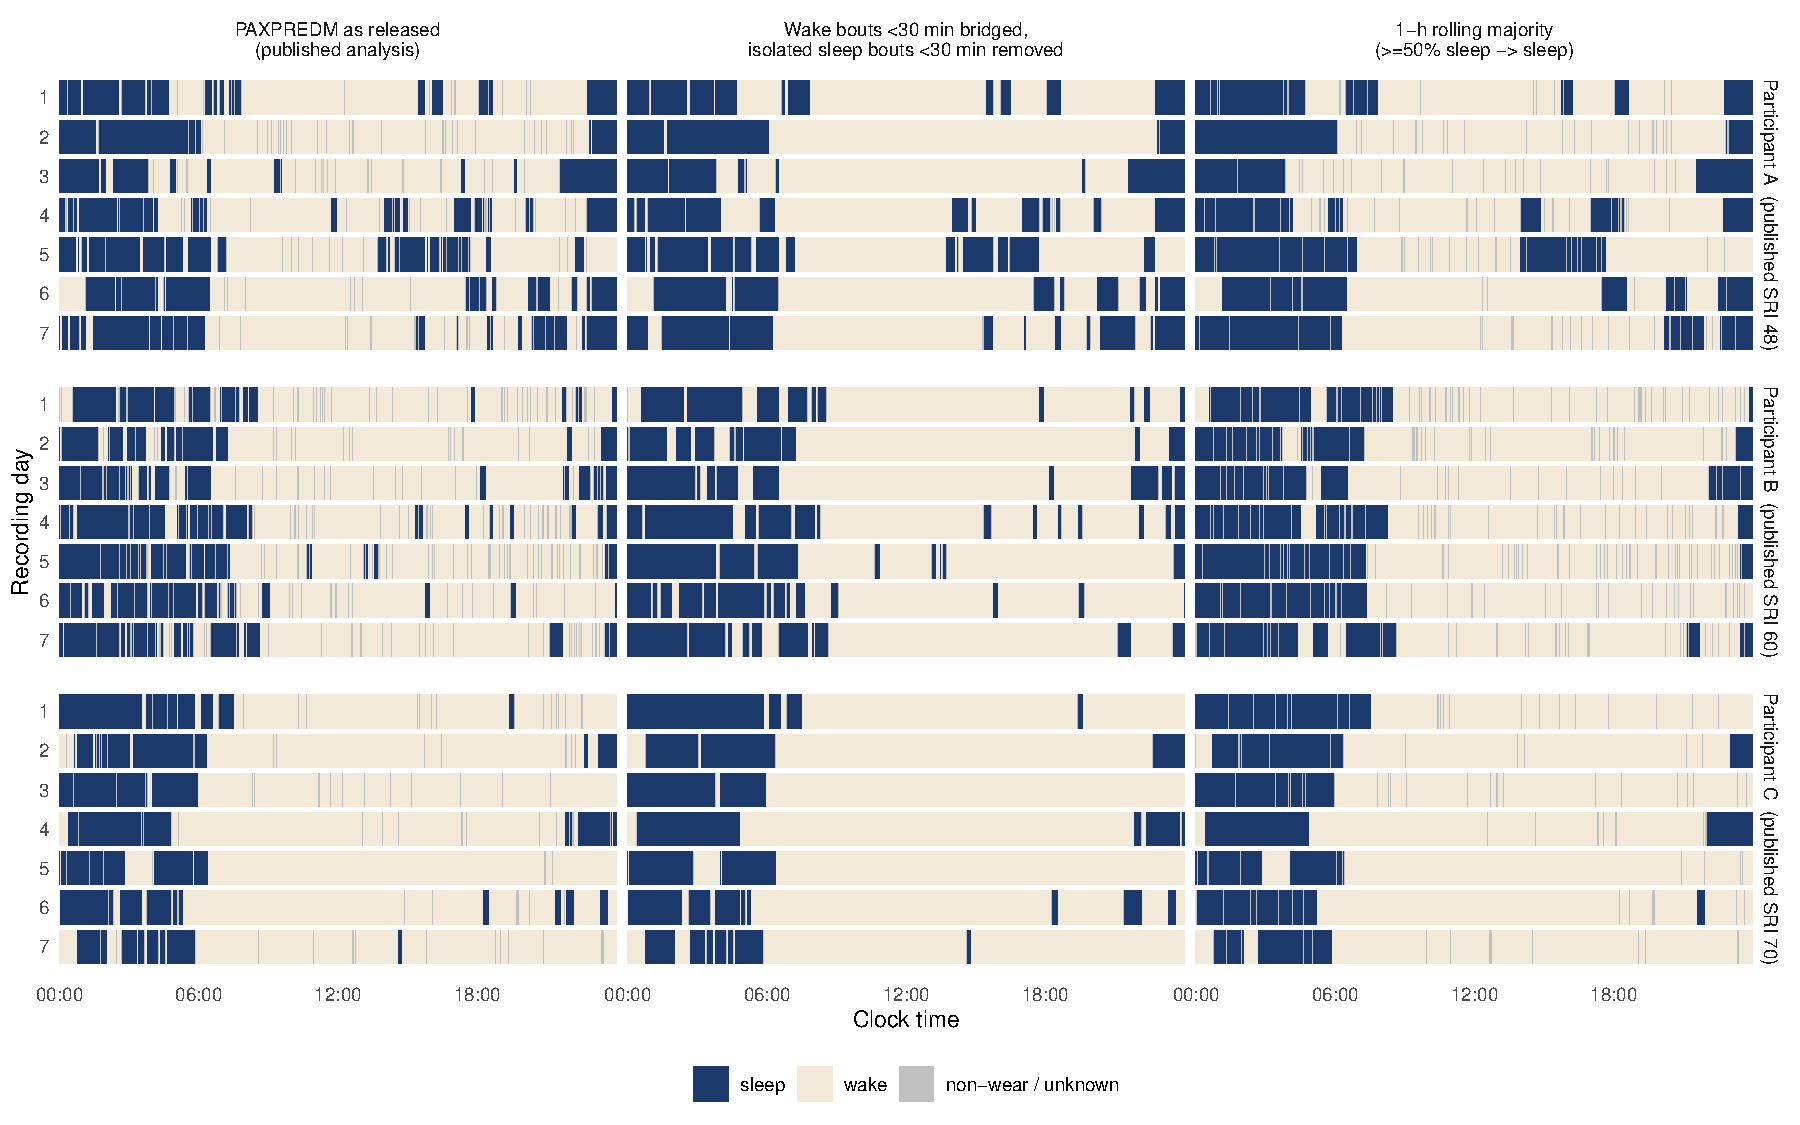
\includegraphics[width=\textwidth]{figures/fig_examples_raw_vs_bridged.pdf}
\caption{Three participants of the 2013--2014 cycle with seven complete recording days, at the 25th, 50th and 75th percentile of the published SRI, shown as released (left), with awakenings shorter than 30 minutes bridged and isolated sleep bouts shorter than 30 minutes removed (middle), and after the 1-h (61-minute) rolling majority filter (right). Navy, sleep; cream, wake; grey, non-wear or unknown.}
\label{fig:rasters}
\end{figure}

\subsection{Calculators on the same input and smoothed input variants}
\label{sec:inputresults}
Given the same timeline, \texttt{GGIR} and the Phillips formula differed by $0.08$ points on average (SD of the difference $2.0$, $r=0.993$) and placed 95\% of participants in the same SRI quintile. \texttt{sleepreg} differed from the formula by $0.02$ to $0.03$ points (SD $0.3$ and $1.7$, $r \geq 0.995$). The agreement held for participants with and without seven consecutive recorded days and for every smoothed input
(Table~\ref{tab:grid}, Supplementary Figure~S4). The packages differed in the number of participants they scored: \texttt{sleepreg} returned no value for 48\% of the 7085
participants at its default and for 25\% at three days, because each excluded
calendar day removes two of its noon-to-noon days, whereas \texttt{GGIR} returned a value for all but 12 to 14 participants, depending on the input. Every smoothing variant raised
the SRI. The median of $61.3$ on the released series rose to between $67.6$
and $69.7$ under the rolling majority, the 80\% rule and the bridging rule
and to $75.5$ with the main sleep period alone, while the mean number of
transitions fell from $17.7$ per day to between $2.1$ and $4.5$
(Table~\ref{tab:grid}, Supplementary Figure~S3 and Section~5).

\begin{table}[t]
\centering
\caption{Median SRI by input variant and calculator (7085 participants, of whom the Phillips formula scores 7076, \texttt{GGIR} 7071 to 7073 and \texttt{sleepreg} the numbers in parentheses at its default minimum of five comparison days and at three), with the Pearson correlation of each
package with the Phillips formula on the same input (for \texttt{sleepreg} at
three days).}
\label{tab:grid}
\setlength{\tabcolsep}{4pt}
\resizebox{\textwidth}{!}{
\begin{tabular}{lcccccc}
\toprule
Input & Phillips formula & \texttt{GGIR} & $r$ & \texttt{sleepreg}, 5 days ($n$) & \texttt{sleepreg}, 3 days ($n$) & $r$ \\
\midrule
Released classification, unsmoothed & 61.3 & 61.4 & 0.993 & 61.0 (3673) & 61.0 (5342) & 0.995 \\
Rolling majority, 1 h & 69.1 & 69.4 & 0.992 & 69.1 (3673) & 69.0 (5342) & 0.994 \\
\texttt{GGIR} SRI1 smoothing, 1 h, 80\% & 69.7 & 69.8 & 0.988 & 69.8 (3673) & 69.5 (5342) & 0.992 \\
Awakenings $<$30 min bridged & 67.6 & 67.8 & 0.994 & 67.0 (3854) & 67.3 (5423) & 0.995 \\
Main sleep period only & 75.5 & 75.7 & 0.990 & 75.8 (3854) & 75.8 (5423) & 0.991 \\
\bottomrule
\end{tabular}
}
\end{table}

\subsection{Recording gaps}
\label{sec:gapresults}
On the synthetic recordings the four implementations returned the known SRI of the five deterministic patterns to within $0.4$ points and placed the random pattern less than one point from zero. On the 300 NHANES recordings with seven consecutive days and the fewest missing minutes they agreed to $0.02$ points (Supplementary
Section~4, Table~S3). With one middle
day retained as missing minutes, the formula and \texttt{GGIR} agreed
($68.75$) and \texttt{sleepreg} returned no value at its default minimum of
comparison days. With the day deleted from the series, the same recording gave
$71.94$ from \texttt{GGIR}, which compared two days 48\,h apart, and
$35.18$ from \texttt{sleepreg}, which stores a series as the times of its
sleep/wake changes and so carries the last state over the deleted day, and
neither package issued a warning (Supplementary
Section~4).

\subsection{Derivation from the raw signal}
\label{sec:rawresults}
On the same participants, days and minutes (the \rawNsample{} participants of the random sample with all four series), each derived series scored higher than the released classification (Table~\ref{tab:rawsri}, Figure~\ref{fig:rawderiv}). The mean
SRI was \rawPaxpredmSriMean{} for \texttt{PAXPREDM}, \rawGgirSibSriMean{} for
\texttt{GGIR} SIB, \rawGgirSptSriMean{} for \texttt{GGIR} SPT and
\rawSwanSriMean{} for SWaN, with mean paired differences from
\texttt{PAXPREDM} of \rawGgirSibDiffMean{}
\CI{\rawGgirSibDiffLo}{\rawGgirSibDiffHi}, \rawGgirSptDiffMean{}
\CI{\rawGgirSptDiffLo}{\rawGgirSptDiffHi} and \rawSwanDiffMean{}
\CI{\rawSwanDiffLo}{\rawSwanDiffHi} points. The released classification changed
state a mean of \rawPaxpredmTransDay{} times per participant-day and labelled
\rawPaxpredmSleepMinDay{} minutes per day as sleep. SWaN, run on the same signal, changed state \rawSwanTransDay{} times per day with \rawSwanSleepMinDay{} minutes of sleep. The \texttt{GGIR} sleep period changed state \rawGgirSptTransDay{} times with \rawGgirSptSleepMinDay{} minutes.
\texttt{GGIR} SIB changed state slightly more often than the released
classification (\rawGgirSibTransDay{} times per day), because sustained inactivity bouts alternate with movement inside the sleep period. Its SRI was still \rawGgirSibDiffMean{} points higher. Minute by minute, the derived series
agreed with the released classification in \rawGgirSibAgreeAll{} to
\rawSwanAgreeAll\% of the minutes (kappa \rawGgirSibKappaAll{} to
\rawSwanKappaAll), in \rawGgirSibAgreeIsm{} to \rawSwanAgreeIsm\% of the
minutes recorded at least half in ISM and in \rawGgirSptAgreeNon{} to
\rawGgirSibAgreeNon\% of the other minutes. The summaries after the first 500 participants of the random order differed from these by less than a point (Supplementary Table~S6, Figure~S5). The sensitivity analysis with each series' own missing minutes is given in Supplementary Section~7.

\begin{table}[t]
\centering
\caption{The released classification and the three series derived from the raw
signal on the same participants, days and minutes (random sample,
$n=\rawNsample$). SRI by the Phillips formula. The difference is the mean paired difference from \texttt{PAXPREDM} with its 95\% bootstrap interval. Agreement is the share of minutes with the same label among the minutes that
\texttt{PAXPREDM} labels wake or sleep, overall and by whether at least half of
the minute was recorded in idle sleep mode (ISM), with Cohen's kappa in
parentheses.}
\label{tab:rawsri}
\setlength{\tabcolsep}{4pt}
\resizebox{\textwidth}{!}{
\begin{tabular}{lcccccccc}
\toprule
 & \multicolumn{2}{c}{SRI} & & Transitions & Sleep & \multicolumn{3}{c}{Agreement with \texttt{PAXPREDM}, \% (kappa)} \\
\cmidrule(lr){2-3}\cmidrule(lr){7-9}
Series & Mean (SD) & Median & Difference (95\% CI) & per day, mean & min/day, mean & All minutes & ISM & Not ISM \\
\midrule
\texttt{PAXPREDM} & \rawPaxpredmSriMean{} (\rawPaxpredmSriSd) & \rawPaxpredmSriMedian & --- & \rawPaxpredmTransDay & \rawPaxpredmSleepMinDay & --- & --- & --- \\
\texttt{GGIR} SIB & \rawGgirSibSriMean{} (\rawGgirSibSriSd) & \rawGgirSibSriMedian & \rawGgirSibDiffMean{} (\rawGgirSibDiffLo, \rawGgirSibDiffHi) & \rawGgirSibTransDay & \rawGgirSibSleepMinDay & \rawGgirSibAgreeAll{} (\rawGgirSibKappaAll) & \rawGgirSibAgreeIsm{} (\rawGgirSibKappaIsm) & \rawGgirSibAgreeNon{} (\rawGgirSibKappaNon) \\
\texttt{GGIR} SPT & \rawGgirSptSriMean{} (\rawGgirSptSriSd) & \rawGgirSptSriMedian & \rawGgirSptDiffMean{} (\rawGgirSptDiffLo, \rawGgirSptDiffHi) & \rawGgirSptTransDay & \rawGgirSptSleepMinDay & \rawGgirSptAgreeAll{} (\rawGgirSptKappaAll) & \rawGgirSptAgreeIsm{} (\rawGgirSptKappaIsm) & \rawGgirSptAgreeNon{} (\rawGgirSptKappaNon) \\
SWaN & \rawSwanSriMean{} (\rawSwanSriSd) & \rawSwanSriMedian & \rawSwanDiffMean{} (\rawSwanDiffLo, \rawSwanDiffHi) & \rawSwanTransDay & \rawSwanSleepMinDay & \rawSwanAgreeAll{} (\rawSwanKappaAll) & \rawSwanAgreeIsm{} (\rawSwanKappaIsm) & \rawSwanAgreeNon{} (\rawSwanKappaNon) \\
\bottomrule
\end{tabular}
}
\end{table}

\begin{figure}[t]
\centering
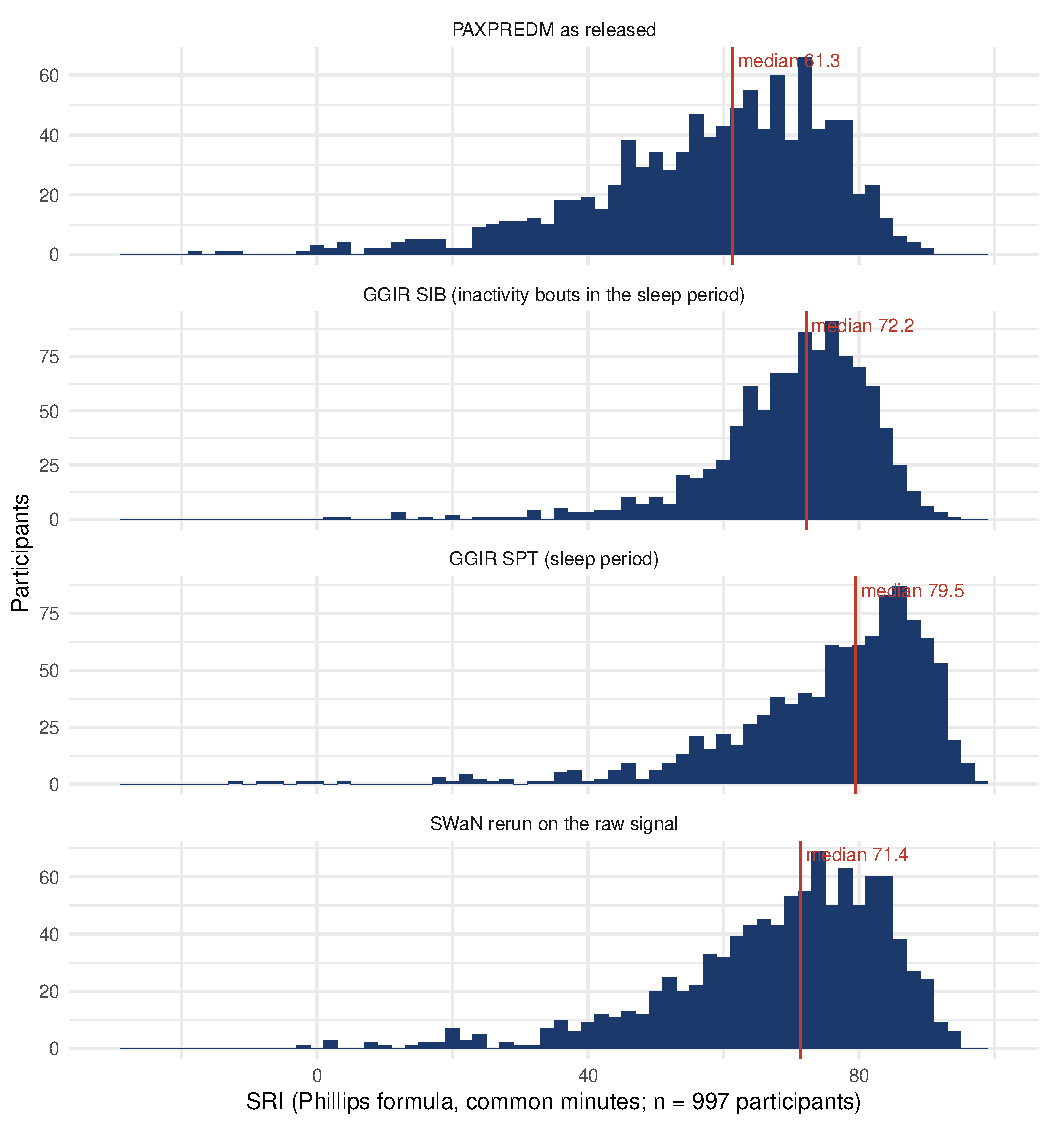
\includegraphics[width=0.7\textwidth]{figures/fig_sri_by_derivation.pdf}
\caption{Distribution of the SRI (Phillips formula on the minutes labelled in both series) for
the released classification and the three series derived from the raw signal
in the random sample ($n=\rawNsample$), with medians.}
\label{fig:rawderiv}
\end{figure}

\subsection{Association with BMI}
\label{sec:rawassoc}
With Models 1 to 3 of the earlier study (its Table~3), the fully adjusted
top-versus-bottom quintile factor on BMI was $0.955$ \CI{0.936}{0.976} on the
released series and $0.963$ to $0.972$ on the smoothed series
(Figure~\ref{fig:forestgrid}, Supplementary Table~S4). In women it was $0.922$
to $0.946$, in men $0.987$ to $1.002$. Expressed as the percentage difference in BMI between the top and bottom SRI quintile, the fully adjusted factor was $-4.5\%$ on the released series and $-2.8\%$ to $-3.7\%$ after smoothing. The factors from \texttt{GGIR}
differed from those of the formula by at most $0.002$, those from
\texttt{sleepreg} were $0.009$ to $0.020$ lower because of its smaller sample
(Supplementary Section~5).

In Model 4, the factors of the twelve race/ethnicity and sex groups on the
published SRI differed from those of the earlier study by at most
\mfourPubMaxDiffOrig{} (its Table~3 reports bootstrap means). The pattern
persisted under every input: in each race/ethnicity group, women had a
lower factor than men in \mfourWomenBelowMen{} comparisons (six groups, six
inputs). Among the five larger race/ethnicity groups the lowest factors were those of non-Hispanic White women, \mfourNhwWomenRelEst{} \CI{\mfourNhwWomenRelLo}{\mfourNhwWomenRelHi} on the released series and \mfourNhwWomenSptEst{} \CI{\mfourNhwWomenSptLo}{\mfourNhwWomenSptHi} with the main-sleep-period input. The smallest group, other race/ethnicity including multiracial (\mfourOthWomenN{} women), had lower point estimates with wide intervals (\mfourOthWomenRelEst{} \CI{\mfourOthWomenRelLo}{\mfourOthWomenRelHi} on the released series). The highest factors were those of Mexican American and non-Hispanic Black men (\mfourMexMenRelEst{} and \mfourNhbMenRelEst{} on the released series). Smoothing moved the group factors by $\mfourShiftLo$ to $\mfourShiftHi$
(Supplementary Section~8, Table~S8, Figures~S6 and S7). \texttt{GGIR} agreed with the formula to \mfourMaxDiffGgir{} or less in every group and input. \texttt{sleepreg} differed by up to \mfourMaxDiffSleepregFive{} in the
smallest groups because of its smaller sample.

\begin{figure}[t]
\centering
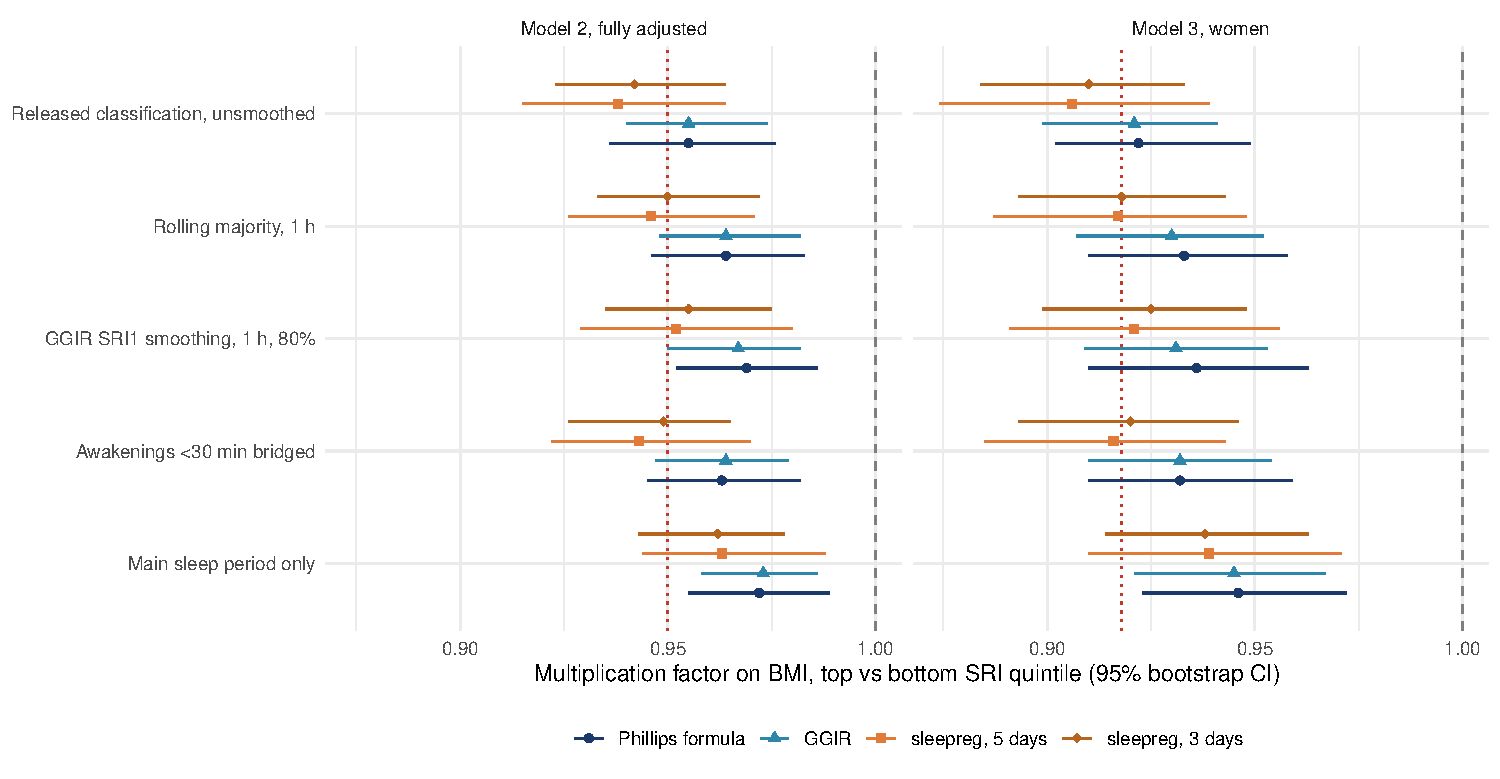
\includegraphics[width=\textwidth]{figures/fig_forest_grid.pdf}
\caption{SRI--BMI multiplication factor (top versus bottom SRI quintile) by
input variant and calculator, with 95\% bootstrap intervals; left, fully
adjusted model; right, women. The dotted red line marks the published value
and the dashed line no association. \texttt{sleepreg} estimates rest on the
participants for whom it returned a score (5 days: $n=3673$ to $3854$; 3
days: $5342$ to $5423$). All inputs are the released classification and its smoothed versions in the published sample. The series derived anew from the raw signal are compared with these inputs on the same participants in Table~\ref{tab:rawassoc}. The estimates are listed in Supplementary Table~S4.}
\label{fig:forestgrid}
\end{figure}

On the \rawModelN{} participants of the random sample, the released
classification gave a fully adjusted factor of \rawPaxpredmMBEst{}
\CI{\rawPaxpredmMBLo}{\rawPaxpredmMBHi}. The derived series gave \rawGgirSibMBEst{} \CI{\rawGgirSibMBLo}{\rawGgirSibMBHi} for \texttt{GGIR} SIB, \rawGgirSptMBEst{} \CI{\rawGgirSptMBLo}{\rawGgirSptMBHi} for
\texttt{GGIR} SPT and \rawSwanMBEst{} \CI{\rawSwanMBLo}{\rawSwanMBHi} for SWaN (Table~\ref{tab:rawassoc}). On the same participants, the four smoothed versions of the released classification gave \rawSmoothedMBMin{} to \rawSmoothedMBMax{}, above the factor of the released classification as in the published sample. Divided by the factor of the released classification in the same bootstrap resamples, the factors of the derived series gave ratios of \rawGgirSibMBRatioEst{} \CI{\rawGgirSibMBRatioLo}{\rawGgirSibMBRatioHi}, \rawGgirSptMBRatioEst{} \CI{\rawGgirSptMBRatioLo}{\rawGgirSptMBRatioHi} and \rawSwanMBRatioEst{} \CI{\rawSwanMBRatioLo}{\rawSwanMBRatioHi}, where a ratio above $1$ means a weaker inverse association. The weaker association is not an effect of the narrower quintile contrast of the derived series: per 10 SRI points, the BMI change was $\rawPaxpredmMBPerTenEst$\% for the released classification and $\rawSwanMBPerTenEst$\% to $\rawGgirSibMBPerTenEst$\% for the derived series (Supplementary Section~7). The sex
pattern of the earlier study appeared in every series, with point estimates
below one in women and above one in men (Table~\ref{tab:rawassoc}). The sensitivity analysis with each series' own
missing minutes gave factors that differed from these by at most $0.01$
(Supplementary Table~S7).
Model 4 on the random sample, with \mfourRawNmin{} to \mfourRawNmax{}
participants per race/ethnicity and sex group, kept the sex pattern in every
series (women below men in all six groups for each of the four series) with wide intervals (widths \mfourRawWidthMin{} to \mfourRawWidthMax{}, Supplementary Table~S9).

Figure~\ref{fig:cidance} shows the intervals of the 20 samples simulated from
the fitted models. With the fully adjusted factor fixed at \simTwoTruth{}, the
point estimates ranged from \simTwoMfMin{} to \simTwoMfMax{} and no 95\% interval reached above \simTwoHiMax{}. The 95\% intervals contained the true factor in \simTwoCoverNinetyFive{} of 20 samples and the
99\% intervals in \simTwoCoverNinetyNine{}. For women (true factor
\simThreeWTruth), the point estimates ranged from \simThreeWMfMin{} to \simThreeWMfMax{}. The 95\% intervals contained the true factor in \simThreeWCoverNinetyFive{} of 20 samples, the 99\% intervals in
\simThreeWCoverNinetyNine{}.

\begin{landscape}
\begin{table}[htbp]
\centering
\caption{SRI--BMI multiplication factor (top versus bottom SRI quintile) on the same \rawModelN{} participants (random sample) for the released classification, its four smoothed versions (the inputs of Figure~\ref{fig:forestgrid}) and the three series derived anew from the raw signal (survey-weighted Models 1 to 3 of the earlier study, its Table~3; 95\% bootstrap intervals).
$\Delta$SRI is the median SRI difference between the top and bottom quintile of
each series. Model~1 adjusts for age and sex, Model~2 is fully adjusted, Model~3
adds a sex $\times$ SRI interaction. The last column is the ratio of the Model~2 factor to that of the unsmoothed released classification, formed in the same bootstrap resamples. Model~4, which gives one factor per race/ethnicity and sex group, is in Supplementary Table~S9.}
\label{tab:rawassoc}
\footnotesize\setlength{\tabcolsep}{2pt}
\begin{tabular}{lcccccc}
\toprule
Series & $\Delta$SRI & Model 1 (age, sex) & Model 2 (fully adjusted) & Model 3, women & Model 3, men & Ratio to released (Model 2) \\
\midrule
\multicolumn{7}{l}{\emph{Released classification (Phillips formula) and its smoothed versions}} \\
Released classification, unsmoothed & \rawPaxpredmMBDSri & \rawPaxpredmMAEst{} (\rawPaxpredmMALo, \rawPaxpredmMAHi) & \rawPaxpredmMBEst{} (\rawPaxpredmMBLo, \rawPaxpredmMBHi) & \rawPaxpredmMCotherEst{} (\rawPaxpredmMCotherLo, \rawPaxpredmMCotherHi) & \rawPaxpredmMCrefEst{} (\rawPaxpredmMCrefLo, \rawPaxpredmMCrefHi) & --- \\
Rolling majority, 1 h & \rawMajMBDSri & \rawMajMAEst{} (\rawMajMALo, \rawMajMAHi) & \rawMajMBEst{} (\rawMajMBLo, \rawMajMBHi) & \rawMajMCotherEst{} (\rawMajMCotherLo, \rawMajMCotherHi) & \rawMajMCrefEst{} (\rawMajMCrefLo, \rawMajMCrefHi) & \rawMajMBRatioEst{} (\rawMajMBRatioLo, \rawMajMBRatioHi) \\
\texttt{GGIR} SRI1 smoothing, 1 h, 80\% & \rawGgirsmMBDSri & \rawGgirsmMAEst{} (\rawGgirsmMALo, \rawGgirsmMAHi) & \rawGgirsmMBEst{} (\rawGgirsmMBLo, \rawGgirsmMBHi) & \rawGgirsmMCotherEst{} (\rawGgirsmMCotherLo, \rawGgirsmMCotherHi) & \rawGgirsmMCrefEst{} (\rawGgirsmMCrefLo, \rawGgirsmMCrefHi) & \rawGgirsmMBRatioEst{} (\rawGgirsmMBRatioLo, \rawGgirsmMBRatioHi) \\
Awakenings $<$30 min bridged & \rawBridgeMBDSri & \rawBridgeMAEst{} (\rawBridgeMALo, \rawBridgeMAHi) & \rawBridgeMBEst{} (\rawBridgeMBLo, \rawBridgeMBHi) & \rawBridgeMCotherEst{} (\rawBridgeMCotherLo, \rawBridgeMCotherHi) & \rawBridgeMCrefEst{} (\rawBridgeMCrefLo, \rawBridgeMCrefHi) & \rawBridgeMBRatioEst{} (\rawBridgeMBRatioLo, \rawBridgeMBRatioHi) \\
Main sleep period only & \rawSptMBDSri & \rawSptMAEst{} (\rawSptMALo, \rawSptMAHi) & \rawSptMBEst{} (\rawSptMBLo, \rawSptMBHi) & \rawSptMCotherEst{} (\rawSptMCotherLo, \rawSptMCotherHi) & \rawSptMCrefEst{} (\rawSptMCrefLo, \rawSptMCrefHi) & \rawSptMBRatioEst{} (\rawSptMBRatioLo, \rawSptMBRatioHi) \\
\midrule
\multicolumn{7}{l}{\emph{Series derived anew from the raw signal}} \\
\texttt{GGIR} SIB & \rawGgirSibMBDSri & \rawGgirSibMAEst{} (\rawGgirSibMALo, \rawGgirSibMAHi) & \rawGgirSibMBEst{} (\rawGgirSibMBLo, \rawGgirSibMBHi) & \rawGgirSibMCotherEst{} (\rawGgirSibMCotherLo, \rawGgirSibMCotherHi) & \rawGgirSibMCrefEst{} (\rawGgirSibMCrefLo, \rawGgirSibMCrefHi) & \rawGgirSibMBRatioEst{} (\rawGgirSibMBRatioLo, \rawGgirSibMBRatioHi) \\
\texttt{GGIR} SPT & \rawGgirSptMBDSri & \rawGgirSptMAEst{} (\rawGgirSptMALo, \rawGgirSptMAHi) & \rawGgirSptMBEst{} (\rawGgirSptMBLo, \rawGgirSptMBHi) & \rawGgirSptMCotherEst{} (\rawGgirSptMCotherLo, \rawGgirSptMCotherHi) & \rawGgirSptMCrefEst{} (\rawGgirSptMCrefLo, \rawGgirSptMCrefHi) & \rawGgirSptMBRatioEst{} (\rawGgirSptMBRatioLo, \rawGgirSptMBRatioHi) \\
SWaN & \rawSwanMBDSri & \rawSwanMAEst{} (\rawSwanMALo, \rawSwanMAHi) & \rawSwanMBEst{} (\rawSwanMBLo, \rawSwanMBHi) & \rawSwanMCotherEst{} (\rawSwanMCotherLo, \rawSwanMCotherHi) & \rawSwanMCrefEst{} (\rawSwanMCrefLo, \rawSwanMCrefHi) & \rawSwanMBRatioEst{} (\rawSwanMBRatioLo, \rawSwanMBRatioHi) \\
\bottomrule
\end{tabular}
\end{table}
\end{landscape}

\begin{figure}[t]
\centering
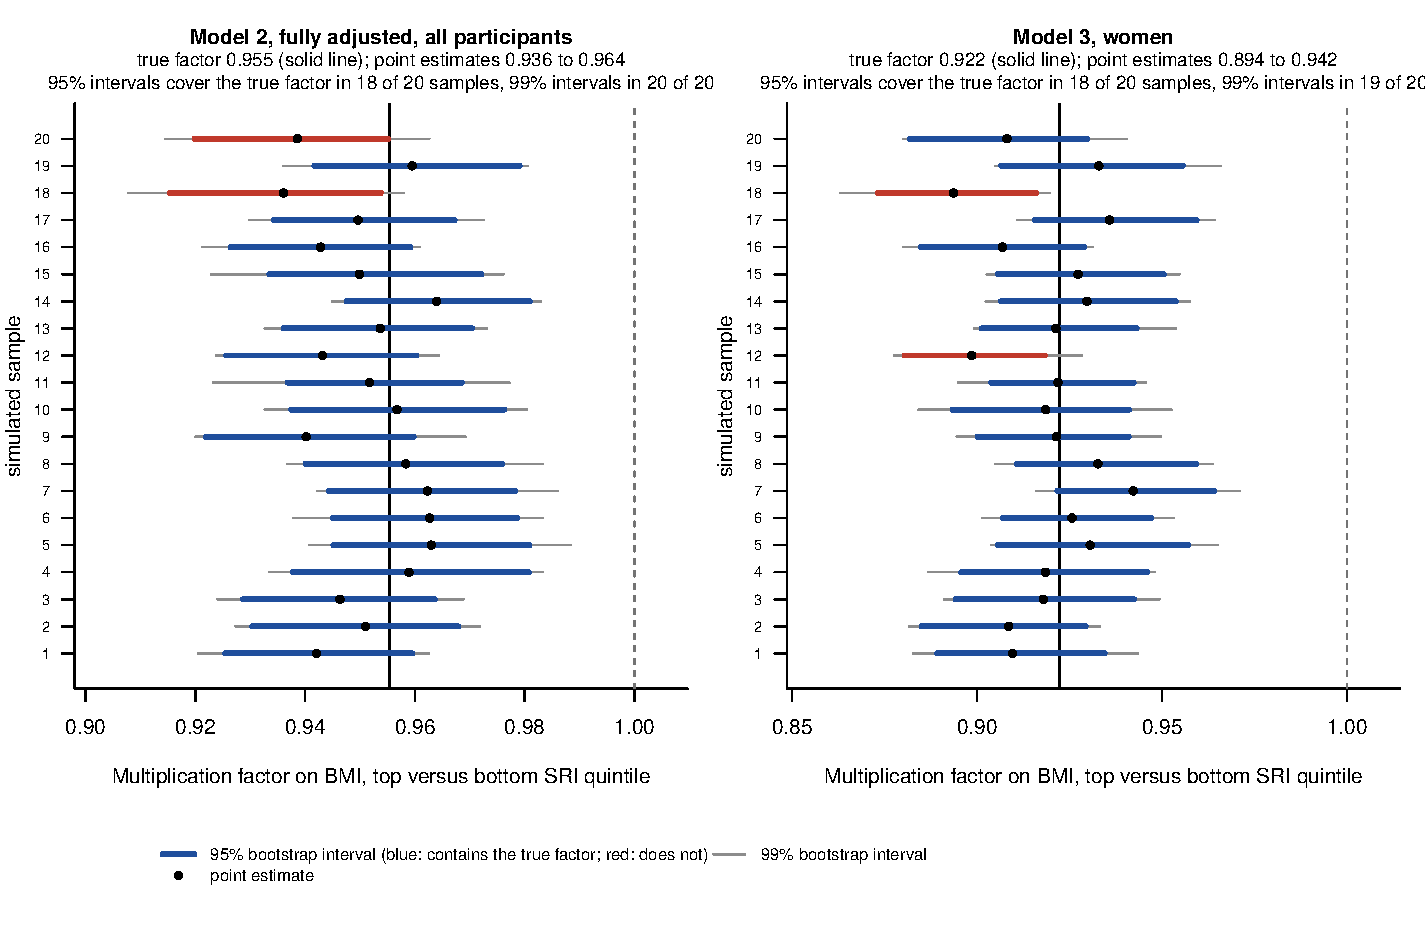
\includegraphics[width=\textwidth]{figures/fig_ci_dance.pdf}
\caption{Twenty samples simulated from the fitted models on the released
series, with the true multiplication factor known (solid line): point
estimates with 95\% (thick) and 99\% (thin) bootstrap intervals of the
SRI--BMI factor, top versus bottom SRI quintile; left, fully adjusted model;
right, women. The dashed grey line marks no association. A 95\% interval drawn in red does not contain the true factor.}
\label{fig:cidance}
\end{figure}

\section{Discussion}

The sleep/wake classification released with NHANES 2011--2014 is highly fragmented. Any SRI computed from it, by any calculator, is the SRI of a fragmented series. The unweighted median of the published values, $61.5$, should be read in this light. Smoothing raised the median to between $67.6$ and $75.5$, closer
to the medians of $74.7$ and $81$ reported for epoch series derived with a
sleep-period detection step [3, 9]. The series derived anew from the raw signal of a random sample scored \rawSwanDiffMean{} to \rawGgirSptDiffMean{} points above the released
classification. The calculators themselves agreed on the same series. Under every smoothed version and every calculator the inverse SRI--BMI association kept its direction. With the Phillips formula and \texttt{GGIR} it lost a fifth to two fifths of its size. With the series derived anew from the raw signal the point estimates moved close to no association: the fully adjusted multiplication factor (Model 2 in Table~\ref{tab:rawassoc}) moved from \rawPaxpredmMBEst{} to between \rawSwanMBEst{} and \rawGgirSibMBEst{}, where $1$ means no association, with 95\% intervals that reach from a small inverse association (lower limits \rawSwanMBLo{} to \rawGgirSibMBLo{}, just above the published $0.950$) to a small positive one (upper limits \rawSwanMBHi{} to \rawGgirSibMBHi{}).

\subsection{Fragmentation of the input and the level of the SRI}
The released series shows a main sleep period at the expected time of day,
cut into short pieces by brief awakenings and unknown epochs, with scattered
short sleep bouts during the day (Figure~\ref{fig:rasters}). Fragmentation
lowers the SRI because the index counts the epoch pairs 24\,h apart that
are in the same state. A brief awakening or an unknown minute inside the sleep
period that does not recur at the same clock time on the next night turns matching pairs into mismatches, as does a short daytime sleep bout on one day only. The classifier behind \texttt{PAXPREDM} [10]
labels 30-second windows and returns no consolidated sleep period. The
post-processing described in the survey documentation is limited to minimum
durations of 3 minutes for wake and 10 minutes for sleep and non-wear and to
an orientation rule [16]. The
present data cannot decide which smoothing is appropriate. The rolling
majority and the bridging rule leave total sleep almost unchanged, the 80\%
rule removes approximately 100 minutes of sleep per day, and the main-sleep-period
rule discards the naps that the SRI as defined by Phillips et al. [1]
includes. The four variants do show that the smoothing decision is at least as important a
reporting item as the calculator: it moved the level by up to 14 points and
the effect size by up to two fifths. The spread of reported NHANES SRIs, from
$78.1$ [7] to $63.0$ [8], is about as wide,
and neither analysis published its code.

\subsection{Calculators, gaps and defaults}
Czeisler et al. [20] found score differences of approximately 20 points between
\texttt{GGIR} and \texttt{sleepreg} in the UK Biobank, where mortality studies
based on \texttt{sleepreg} [18] and on \texttt{GGIR} [19] differ in effect size. In their comparison the packages shared
\texttt{GGIR}'s epoch states, but \texttt{sleepreg} then re-handled naps and
awakenings with its own rules. In the present analysis that re-handling did
not run, the series was identical down to the representation of its gaps, and
the packages agreed. The two findings are compatible if the divergence in the
UK Biobank arises in the derivation of the sleep/wake series, since the
arithmetic of the index is the same in all packages. The packages differed at gaps in the data, where the index compares each epoch with the epoch exactly 24\,h later and has no pair when either is missing. A day deleted from a series instead of marked as
missing is bridged without warning: \texttt{GGIR} pairs the date before the
gap with the next date present, and \texttt{sleepreg} extends the last state
over the gap. \texttt{sleepreg} also blanks any noon-to-noon day with more
than 6\,h missing, so that a single excluded calendar day costs two of
its comparison days. With the default minimum of five, no NHANES participant with a gap received a score. The 48\% lost in this way were selected by wear behaviour, since only participants with seven consecutive recorded days remain, and are not a random subset. None of these behaviours is an
error in packages written for continuous raw recordings, but each is
undocumented for a pre-classified series with excluded days, which is how a
survey such as NHANES is used.

\subsection{Derivation from the raw signal and the association with BMI}
Run on the raw signal of the same participants, the public code of SWaN
produced a series with \rawSwanTransDay{} transitions per day where the released
classification has \rawPaxpredmTransDay. The two series agree in \rawSwanAgreeAll\% of the minutes. The disagreement is concentrated in the minutes recorded in idle sleep mode (\rawSwanAgreeIsm\% against
\rawSwanAgreeNon\%). Two differences between the runs can account for this:
the released classification was produced with a procedure that replaces the
ISM stretches by the 10 seconds of signal that precede them [16], whereas the rerun used the signal as recorded,
and the version of the code behind the release is not documented. The
fragmentation of the released series therefore does not follow from the public SWaN code. It belongs to the run that produced the release. The
concentration of the disagreement in ISM minutes is consistent with a role of
the ISM replacement, although the \texttt{GGIR} series, which involve no such
replacement either, show the same concentration.

The association with BMI weakened with the derived series more than with the smoothed variants: on the same \rawModelN{} participants, the smoothed versions of the released classification gave fully adjusted factors of \rawSmoothedMBMin{} to \rawSmoothedMBMax{} and the derived series \rawSwanMBEst{} to \rawGgirSibMBEst{} (Table~\ref{tab:rawassoc}). The ratios of the fully adjusted factors to that of the released classification were \rawSwanMBRatioEst{} to \rawGgirSibMBRatioEst. The factors themselves, \rawSwanMBEst{} to \rawGgirSibMBEst, are compatible with no association as well as with a small inverse or a small positive one. Two readings remain open. If the derived series measure the construct with less noise, the published association was inflated by an error in the released series that is itself related to adiposity (daytime sleep, movement during sleep or non-wear labelled as sleep). Random error alone would have attenuated it, as regression dilution predicts. If the fragmentation carries information about sleep that is itself related to BMI,
the derived series remove it. The present data cannot separate the two. They
show that the size of the association depends on the processing pipeline more
than on the calculator, with the fully adjusted factor, expressed as the percentage difference in BMI between the top and bottom quintile, from approximately $-5\%$ for the released classification ($-4.8\%$ on the same participants, $-4.5\%$ in the published sample) to approximately zero for the series derived anew from the signal (Table~\ref{tab:rawassoc}, Supplementary Table~S4). A reader who classifies results by whether the 95\% interval includes 1 would reach opposite conclusions from the same participants, an inverse association with the released classification and none with the derived series (Table~\ref{tab:rawassoc}). This reading is the one that Wasserstein et al. [23] advise against: an interval shows the effect sizes most compatible with the data under the model. Whether it includes 1 is not a result.

For the earlier study itself, the rebuilt series moved the fully adjusted
estimate from $0.950$ to $0.955$ and left the sex pattern unchanged. The sex and race/ethnicity pattern of its Model 4 (its Figure~2) persisted under every input (Supplementary Table~S8, Figures~S6 and S7). Its
Methods describe the final state of its code and not the computation behind
its reported values. This difference does not change its conclusions, but it
belongs beside its reported SRI values (Supplementary Section~3).

\subsection{Limitations}
The series was rebuilt from the public files with the filters as published,
whereas the published scores came from earlier states of the processing code. The same-input baseline is hence the formula on the rebuilt series. The two give effect sizes that differ by $0.005$. No reference measure of sleep
exists for these participants, so that the agreement between derivations is a
concordance between algorithms. The sleep
detection of \texttt{GGIR} was developed on other monitors [5, 12] and applied to recordings in idle sleep mode.
The derivation covers a random sample of \rawNsample{} participants, about one
seventh of the published sample, with correspondingly wider intervals. The summaries after the first 500 participants differed by less than a point from
those after 1000 (Supplementary Table~S6). SWaN was run without the ISM
replacement that the survey documentation describes and with the public
version of its code, whose relation to the version behind the release is
unknown. The autocalibration of \texttt{GGIR} depends on the floating-point precision of the processor. The derived series were computed on five platforms. For the 80 participants processed both on the Apple platform and on another machine, the sleep/wake minute labels of all three series were identical (Supplementary Section~7, Table~S5). The
smoothing rules are simple post-processing steps without validation as sleep-period detectors. The main-sleep-period variant changes the construct by removing naps.

\subsection{Reporting items for pre-classified series}
The RIRI statement asks for the data processing tool, the quality control and the additional configurations of an SRI analysis [20]. For a pre-classified series, five details fill these items. (1) How the epoch-level series was derived (classifier,
version, handling of the monitor's idle sleep mode), whether and how it was
smoothed, and its fragmentation (transitions per day, bout lengths). (2) How
excluded minutes and days were passed to the calculator, as missing values or
as deletions, and whether the package's own inclusion criterion was applied to
its day pairs. (3) The minimum-day rule and the analytic sample it leaves. (4)
Effect sizes with compatibility intervals for each processing choice that was
tried. (5) The state of the processing code that produced the reported values,
archived with them. Item (4) asks for the interval as a range of compatible
values. Figure~\ref{fig:cidance} shows why: in 20 samples simulated from the
fitted model, the point estimates moved between \simTwoMfMin{} and
\simTwoMfMax{} and the interval ends by more, while the factor that generated
the data stayed at \simTwoTruth{}. One interval from one sample is one draw
from this variation [17, 21]. The completed RIRI checklist of the present study is Supplementary Table~S1. A
World Sleep Society specification for consumer sleep trackers [22] did not adopt the SRI, citing the lack of a standard computation. It specifies instead that the 30-second sleep/wake/unknown epoch array should be retained. Such an array needs to carry the classification, the smoothing
applied to it, the inclusion filters and the position of its gaps.

\section{Conclusions}
The level of the SRI in NHANES 2011--2014 depended on the sleep/wake input and
only marginally on the calculator. Given the same series, the Phillips formula,
\texttt{GGIR} and \texttt{sleepreg} agreed to 0.1 points. Smoothing the released
classification raised the median SRI from 61 to 68--76. The three series derived
anew from the raw signal scored 10 to 18 points higher than the release, and the
released classification is more fragmented than a classification of the same
signal with the public code of the same algorithm. The inverse SRI--BMI association kept its direction under every smoothed input and, with the Phillips formula and \texttt{GGIR}, lost a fifth to two fifths of its size. With the series derived anew from the raw signal the point estimates moved close to no association, with intervals reaching from a small inverse association near the published value to a small positive one. The packages differ in how they treat a
recording gap. A day deleted instead of marked as missing changes the result
without warning. Studies of the SRI should report the derivation and smoothing
of the series, the treatment of gaps, the minimum-day rule and the remaining
sample. The processing code should be archived with the results.

\section*{List of abbreviations}
\begin{description}\setlength{\itemsep}{0pt}
\item[BMI] body mass index
\item[CI] confidence interval
\item[IQR] interquartile range
\item[ISM] idle sleep mode
\item[MF] multiplication factor
\item[NCHS] National Center for Health Statistics
\item[NHANES] National Health and Nutrition Examination Survey
\item[PAXPREDM] predicted sleep/wake state in the NHANES minute-level accelerometry files
\item[RIRI] Reporting Items for Regularity Indices
\item[SD] standard deviation
\item[SIB] sustained inactivity bout
\item[SPT] sleep period time
\item[SRI] Sleep Regularity Index
\item[SWaN] sleep-wear, wake-wear and nonwear classifier
\end{description}

\section*{Declarations}

\paragraph{Ethics approval and consent to participate.} This is a secondary analysis of
de-identified, publicly available NHANES 2011--2014 data. The NHANES protocol was
approved by the National Center for Health Statistics (NCHS) Research Ethics Review
Board, and all participants provided written informed consent at the time of the
survey. No further ethics approval was required for this re-analysis.

\paragraph{Consent for publication.} Not applicable. The study uses de-identified
public data and reports no individually identifiable information.

\paragraph{Availability of data and materials.} All data are NHANES 2011--2012 and 2013--2014
public-use files of the US National Center for Health Statistics
(\url{https://wwwn.cdc.gov/nchs/nhanes/}): the Physical Activity Monitor minute
and header files (\texttt{PAXMIN}, \texttt{PAXHD}), the raw 80\,Hz
acceleration files (\texttt{PAX80\_G} and \texttt{PAX80\_H}, one archive per
participant, 2.45\,TB in total) and the covariate files of the earlier study.
The companion repository
(\url{https://github.com/jdegenfellner/SRI_BMI_NHANES_2026_reanalysis_public})
contains the code of every step, the analytic covariate data set, the derived
SRI values of every calculator and input variant, the minute-level sleep/wake
series of every derivation, the container definition of the cloud runs and the
code that reproduces the published SRI values exactly. A frozen copy with the
recoded minute files and all intermediate series is archived at Zenodo
(\url{https://doi.org/10.5281/zenodo.23482613}), so that every table and figure can be recomputed from the archived files without any download (run order in \texttt{code/revision\_2026-10/README.md}).

\paragraph{Competing interests.} The author declares no competing interests.

\paragraph{Funding.} The author received no financial support for the research, authorship or publication of this article.

\paragraph{Authors' contributions.} JD conceived the study, performed all analyses,
wrote the manuscript and approved the final version.

\paragraph{Acknowledgements.} The author thanks the NHANES participants and the
National Center for Health Statistics for collecting and releasing the data.

\paragraph{Clinical trial number.} Not applicable.

\paragraph{Use of artificial intelligence.} A large language model (Claude, Anthropic) assisted with drafting and language editing of the manuscript and with writing and executing the analysis code, as stated in the Methods. The author takes full responsibility for the content.

\clearpage
\section*{References}
\begin{sloppypar}
\setlength{\parindent}{0pt}
\raggedright
\hangindent=1.5em \hangafter=1 \noindent 1. Phillips AJK, Clerx WM, O'Brien CS, Sano A, Barger LK, Picard RW, Lockley SW, Klerman EB, Czeisler CA. Irregular sleep/wake patterns are associated with poorer academic performance and delayed circadian and sleep/wake timing. Sci Rep. 2017;7:3216. \url{https://doi.org/10.1038/s41598-017-03171-4}

\hangindent=1.5em \hangafter=1 \noindent 2. Fischer D, Klerman EB, Phillips AJK. Measuring sleep regularity: theoretical properties and practical usage of existing metrics. Sleep. 2021;44(10):zsab103. \url{https://doi.org/10.1093/sleep/zsab103}

\hangindent=1.5em \hangafter=1 \noindent 3. Windred DP, Jones SE, Russell A, Burns AC, Chan P, Weedon MN, Rutter MK, Olivier P, Vetter C, Saxena R, Lane JM, Cain SW, Phillips AJK. Objective assessment of sleep regularity in 60,000 UK Biobank participants using an open-source package. Sleep. 2021;44(12):zsab254. \url{https://doi.org/10.1093/sleep/zsab254}

\hangindent=1.5em \hangafter=1 \noindent 4. Migueles JH, Rowlands AV, Huber F, Sabia S, van Hees VT. GGIR: a research community-driven open source R package for generating physical activity and sleep outcomes from multi-day raw accelerometer data. J Meas Phys Behav. 2019;2(3):188--96. \url{https://doi.org/10.1123/jmpb.2018-0063}

\hangindent=1.5em \hangafter=1 \noindent 5. van Hees VT, Sabia S, Anderson KN, Denton SJ, Oliver J, Catt M, Abell JG, Kivim\"aki M, Trenell MI, Singh-Manoux A. A novel, open access method to assess sleep duration using a wrist-worn accelerometer. PLoS One. 2015;10(11):e0142533. \url{https://doi.org/10.1371/journal.pone.0142533}

\hangindent=1.5em \hangafter=1 \noindent 6. Degenfellner J, Schernhammer ES, Strohmaier S. Sex- and ethnic differences in the cross-sectional association between sleep regularity and obesity among US adults, NHANES 2011--2014. J Biol Rhythms. 2026;41(2):205--18. \url{https://doi.org/10.1177/07487304251391267}

\hangindent=1.5em \hangafter=1 \noindent 7. Wang X, Xu Y, Li X, Mansuri A, McCall WV, Liu Y. Day-to-day deviations in sleep parameters and biological aging: findings from the NHANES 2011--2014. Sleep Health. 2023;9(6):940--6. \url{https://doi.org/10.1016/j.sleh.2023.07.018}

\hangindent=1.5em \hangafter=1 \noindent 8. Yang L, Wallen G, Barb J, Maki K, Farmer N. 0863 Sleep regularity and cardiovascular health among U.S. adults [conference abstract]. Sleep. 2024;47(Suppl 1):A370--1. \url{https://doi.org/10.1093/sleep/zsae067.0863}

\hangindent=1.5em \hangafter=1 \noindent 9. Lunsford-Avery JR, Engelhard MM, Navar AM, Kollins SH. Validation of the sleep regularity index in older adults and associations with cardiometabolic risk. Sci Rep. 2018;8:14158. \url{https://doi.org/10.1038/s41598-018-32402-5}

\hangindent=1.5em \hangafter=1 \noindent 10. Thapa-Chhetry B, Arguello DJ, John D, Intille S. Detecting sleep and nonwear in 24-h wrist accelerometer data from the National Health and Nutrition Examination Survey. Med Sci Sports Exerc. 2022;54(11):1936--46. \url{https://doi.org/10.1249/MSS.0000000000002973}

\hangindent=1.5em \hangafter=1 \noindent 11. National Center for Health Statistics. National Health and Nutrition Examination Survey 2011--2012 data documentation, codebook, and frequencies: physical activity monitor, raw data 80 Hz (PAX80\_G). Hyattsville (MD): Centers for Disease Control and Prevention; 2022. \url{https://wwwn.cdc.gov/Nchs/Data/Nhanes/Public/2011/DataFiles/PAX80_G.htm}

\hangindent=1.5em \hangafter=1 \noindent 12. van Hees VT, Sabia S, Jones SE, Wood AR, Anderson KN, Kivim\"aki M, Frayling TM, Pack AI, Bucan M, Trenell MI, Mazzotti DR, Gehrman PR, Singh-Manoux A, Weedon MN. Estimating sleep parameters using an accelerometer without sleep diary. Sci Rep. 2018;8:12975. \url{https://doi.org/10.1038/s41598-018-31266-z}

\hangindent=1.5em \hangafter=1 \noindent 13. Hammad G, Reyt M, Beliy N, Baillet M, Deantoni M, Lesoinne A, Muto V, Schmidt C. pyActigraphy: open-source python package for actigraphy data visualization and analysis. PLoS Comput Biol. 2021;17(10):e1009514. \url{https://doi.org/10.1371/journal.pcbi.1009514}

\hangindent=1.5em \hangafter=1 \noindent 14. van Hees VT, Fang Z, Langford J, Assah F, Mohammad A, da Silva ICM, Trenell MI, White T, Wareham NJ, Brage S. Autocalibration of accelerometer data for free-living physical activity assessment using local gravity and temperature: an evaluation on four continents. J Appl Physiol (1985). 2014;117(7):738--44. \url{https://doi.org/10.1152/japplphysiol.00421.2014}

\hangindent=1.5em \hangafter=1 \noindent 15. Koffman L, Muschelli J. Minute level step counts and physical activity data from the National Health and Nutrition Examination Survey (NHANES) 2011--2014 (version 1.0.2) [data set]. PhysioNet; 2026. \url{https://doi.org/10.13026/d7sw-f662}

\hangindent=1.5em \hangafter=1 \noindent 16. National Center for Health Statistics. National Health and Nutrition Examination Survey 2011--2012 data documentation, codebook, and frequencies: physical activity monitor, minute (PAXMIN\_G). Hyattsville (MD): Centers for Disease Control and Prevention; 2022. \url{https://wwwn.cdc.gov/Nchs/Data/Nhanes/Public/2011/DataFiles/PAXMIN_G.htm}

\hangindent=1.5em \hangafter=1 \noindent 17. Cumming G. The new statistics: why and how. Psychol Sci. 2014;25(1):7--29. \url{https://doi.org/10.1177/0956797613504966}

\hangindent=1.5em \hangafter=1 \noindent 18. Windred DP, Burns AC, Lane JM, Saxena R, Rutter MK, Cain SW, Phillips AJK. Sleep regularity is a stronger predictor of mortality risk than sleep duration: a prospective cohort study. Sleep. 2024;47(1):zsad253. \url{https://doi.org/10.1093/sleep/zsad253}

\hangindent=1.5em \hangafter=1 \noindent 19. Cribb L, Sha R, Yiallourou S, Grima NA, Cavuoto M, Baril AA, Pase MP. Sleep regularity and mortality: a prospective analysis in the UK Biobank. eLife. 2023;12:RP88359. \url{https://doi.org/10.7554/eLife.88359}

\hangindent=1.5em \hangafter=1 \noindent 20. Czeisler M\'E, Windred DP, Phillips AJK, Sabia S, van Hees VT, Rutter MK, Cain SW. Comparison of Sleep Regularity Index scores calculated by open-source packages and implications for outcomes research: rationale and design of the RIRI statement. Sleep. 2026;49(4):zsaf299. \url{https://doi.org/10.1093/sleep/zsaf299}

\hangindent=1.5em \hangafter=1 \noindent 21. Greenland S, Senn SJ, Rothman KJ, Carlin JB, Poole C, Goodman SN, Altman DG. Statistical tests, P values, confidence intervals, and power: a guide to misinterpretations. Eur J Epidemiol. 2016;31(4):337--50. \url{https://doi.org/10.1007/s10654-016-0149-3}

\hangindent=1.5em \hangafter=1 \noindent 22. Chee MWL, Baumert M, Drummond SPA, Scott H, Goldstein CA, de Zambotti M, Heneghan C, Leota J, Hao S, Cimesa L, Cellini N, Overeem S, Baron KG, Sharafkhaneh A, Penzel T, Kushida CA. Standardizing wearable sleep data for clinical, research, and public health use: a World Sleep Society specification. Sleep Med. 2026;109310. Advance online publication. \url{https://doi.org/10.1016/j.sleep.2026.109310}

\hangindent=1.5em \hangafter=1 \noindent 23. Wasserstein RL, Schirm AL, Lazar NA. Moving to a world beyond ``$p < 0.05$''. Am Stat. 2019;73(sup1):1--19. \url{https://doi.org/10.1080/00031305.2019.1583913}
\end{sloppypar}

\end{document}
